\documentclass[output=paper, colorlinks, citecolor=brown, newtxmath]{langsci/langscibook}
\ChapterDOI{10.5281/zenodo.3764845}
% \bibliography{localbibliography}
% % add all extra packages you need to load to this file  
\usepackage{tabularx} 
\definecolor{lsDOIGray}{cmyk}{0,0,0,0.45}

\usepackage{xassoccnt}
\newcounter{realpage}
\DeclareAssociatedCounters{page}{realpage}
\AtBeginDocument{%
  \stepcounter{realpage}
}

%%%%%%%%%%%%%%%%%%%%%%%%%%%%%%%%%%%%%%%%%%%%%%%%%%%%
%%%           Examples                           %%%
%%%%%%%%%%%%%%%%%%%%%%%%%%%%%%%%%%%%%%%%%%%%%%%%%%%%  
%% if you want the source line of examples to be in italics, uncomment the following line
% \renewcommand{\exfont}{\itshape}
\usepackage{lipsum}
\usepackage{langsci-optional}
\usepackage{./langsci-osl}
\usepackage{langsci-lgr}
\usepackage{langsci-gb4e}
\usepackage{stmaryrd}
\usepackage{pifont} % needed for checkmark \ding{51} and cross \ding{55}
\usepackage[linguistics]{forest}

% ch06
\usepackage[euler]{textgreek}
% ch07
\usepackage{soul}
\usepackage{graphicx}
% ch08, ch14
\usepackage{multicol}
% ch11
\usepackage{fnpct}
% ch13
\usepackage{scrextend}
\usepackage{enumitem}
% ch14
\usepackage{tabto}
\usepackage{multirow}

\usepackage{langsci-cgloss}

% \newcommand{\smiley}{ :) }

% non-italics in examples

\renewcommand{\eachwordone}{\upshape}

% non-italics in examples in footnotes

\renewcommand{\fnexfont}{\footnotesize\upshape}
\renewcommand{\fnglossfont}{\footnotesize\upshape}
\renewcommand{\fntransfont}{\footnotesize\upshape}
\renewcommand{\fnexnrfont}{\fnexfont\upshape}

% chapter03 goncharov

\newcommand{\p}{\textsc{pfv\ }}
\newcommand{\im}{\textsc{ipfv\ }}

\makeatletter
\let\thetitle\@title
\let\theauthor\@author 
\makeatother

\newcommand{\togglepaper}[1][0]{  
  \addbibresource{../localbibliography.bib}  
  \papernote{\scriptsize\normalfont
    \theauthor.
    \thetitle. 
    To appear in: 
    Change Volume Editor \& in localcommands.tex 
    Change volume title in localcommands.tex
    Berlin: Language Science Press. [preliminary page numbering]
  }
  \pagenumbering{roman}
  \setcounter{chapter}{#1}
  \addtocounter{chapter}{-1}
}

\providecommand{\orcid}[1]{}

\title{N-words and NPIs: Between syntax, semantics, and experiments}
\providecommand{\subtitle}[1]{}
\author{Mojmír Dočekal\affiliation{Masaryk University in Brno}}

\abstract{In this paper I experimentally approach the following question: do strict negative concord languages like Czech employ two strategies (syntactic and semantic) to encode negative dependency between a verb and its argument(s) or not? And the answer is: beside the default syntactic strategy (n-words), there is a class of negative dependent expressions which are licensed by semantic rules.

\keywords{n-words, negative polarity items, experiments, neg-raising, Czech}
}


\IfFileExists{../localcommands.tex}{
  % add all extra packages you need to load to this file  
\usepackage{tabularx} 
\definecolor{lsDOIGray}{cmyk}{0,0,0,0.45}

\usepackage{xassoccnt}
\newcounter{realpage}
\DeclareAssociatedCounters{page}{realpage}
\AtBeginDocument{%
  \stepcounter{realpage}
}

%%%%%%%%%%%%%%%%%%%%%%%%%%%%%%%%%%%%%%%%%%%%%%%%%%%%
%%%           Examples                           %%%
%%%%%%%%%%%%%%%%%%%%%%%%%%%%%%%%%%%%%%%%%%%%%%%%%%%%  
%% if you want the source line of examples to be in italics, uncomment the following line
% \renewcommand{\exfont}{\itshape}
\usepackage{lipsum}
\usepackage{langsci-optional}
\usepackage{./langsci-osl}
\usepackage{langsci-lgr}
\usepackage{langsci-gb4e}
\usepackage{stmaryrd}
\usepackage{pifont} % needed for checkmark \ding{51} and cross \ding{55}
\usepackage[linguistics]{forest}

% ch06
\usepackage[euler]{textgreek}
% ch07
\usepackage{soul}
\usepackage{graphicx}
% ch08, ch14
\usepackage{multicol}
% ch11
\usepackage{fnpct}
% ch13
\usepackage{scrextend}
\usepackage{enumitem}
% ch14
\usepackage{tabto}
\usepackage{multirow}

\usepackage{langsci-cgloss}

  \newcommand{\smiley}{ :) }

% non-italics in examples

\renewcommand{\eachwordone}{\upshape}

% non-italics in examples in footnotes

\renewcommand{\fnexfont}{\footnotesize\upshape}
\renewcommand{\fnglossfont}{\footnotesize\upshape}
\renewcommand{\fntransfont}{\footnotesize\upshape}
\renewcommand{\fnexnrfont}{\fnexfont\upshape}

% chapter03 goncharov

\newcommand{\p}{\textsc{pfv\ }}
\newcommand{\im}{\textsc{ipfv\ }}

\makeatletter
\let\thetitle\@title
\let\theauthor\@author 
\makeatother

\newcommand{\togglepaper}[1][0]{  
  \addbibresource{../localbibliography.bib}  
  \papernote{\scriptsize\normalfont
    \theauthor.
    \thetitle. 
    To appear in: 
    Change Volume Editor \& in localcommands.tex 
    Change volume title in localcommands.tex
    Berlin: Language Science Press. [preliminary page numbering]
  }
  \pagenumbering{roman}
  \setcounter{chapter}{#1}
  \addtocounter{chapter}{-1}
}

\providecommand{\orcid}[1]{}
  %% hyphenation points for line breaks
%% Normally, automatic hyphenation in LaTeX is very good
%% If a word is mis-hyphenated, add it to this file
%%
%% add information to TeX file before \begin{document} with:
%% %% hyphenation points for line breaks
%% Normally, automatic hyphenation in LaTeX is very good
%% If a word is mis-hyphenated, add it to this file
%%
%% add information to TeX file before \begin{document} with:
%% %% hyphenation points for line breaks
%% Normally, automatic hyphenation in LaTeX is very good
%% If a word is mis-hyphenated, add it to this file
%%
%% add information to TeX file before \begin{document} with:
%% \include{localhyphenation}
\hyphenation{
Ro-ma-no-va
Isa-čen-ko
}

\hyphenation{
Ro-ma-no-va
Isa-čen-ko
}

\hyphenation{
Ro-ma-no-va
Isa-čen-ko
}

  \togglepaper[2]%%chapternumber
}{}
% \togglepaper[2]

\begin{document}
\maketitle

\il{Czech|(}
\section{Introduction}\label{intro}

In this article I \isi{focus} on a problem of dividing negative dependent expressions into two classes: (i) \textsc{n-words} like \ili{Czech} \textit{nikdo} `nobody' or \ili{Romanian} \textit{nimeni} `nobody' (glossed as \textsc{n-person}) in \REF{ex-1-a}; (ii) \textsc{\isi{negative polarity} items} (NPIs) like \ili{Czech} \textit{sebemenší šance} `slightest chance ' or \ili{Romanian} \textit{vreun} `any' in \REF{ex-1-b}. Despite the long research traditions on both types of expressions (for NPIs see \citealt{heim1984note,ladusaw1992expressing,kadmon1993any,krifka1995semantics,giannakidou1997landscape,lahiri1998focus, gajewski2011licensing,chierchia2013logic,crnivc2014against} among many others; for n-words see \citealt{laka1990negation,zeijlstra2004sentential,zeijlstra2008negative} among others) there is still no consensus on the relationship between the two classes of items.%
\footnote{Both n-words and NPIs are generally grammatical in sentences with a negated \isi{verb}. There are of course language-specific differences, e.g. \ili{English} \isi{NPI} \textit{any} usually cannot appear in \isi{subject position}, \ili{Romanian} \textit{vreun} `any' in \REF{ex-1-b} behaves similarly but many languages allow NPIs to freely occur in \isi{subject position} -- \cite{Blasczak:2001} lists \ili{Hindi}, \ili{Korean}, \ili{Japanese} among many other languages where NPIs are licensed in any position of a sentence with a negated \isi{verb}. Slavic languages discussed in detail further belong to the set of languages allowing NPIs in \isi{subject position}, too.}

\ea \label{ex-1} \ea[]{ \label{ex-1-a} \gll Nimeni nu a venit.\\
\textsc{n-person} not has come\\
\glt `Nobody came.'}
\ex[*]{\label{ex-1-b} \gll Vreun student nu a venit.\\
\textsc{npi} student not has come\\
\glt Intended: `No student did not come.'\\\xspace\hfill (\ili{Romanian}; \citealt[586, 591]{fualuaus2016fragment})}
\z
\z

\noindent Nevertheless, it seems to be settled that the division between n-words and NPIs correlates with the division between syntactic licensing and semantic licensing along the following lines:%

\largerpage
\begin{enumerate}
\def\labelenumi{\arabic{enumi})}
\item
  \textsc{n-words} are syntactically negative dependent expressions;\footnote{This classification is of course very schematic and it can be a bit problematic to apply it to a set of typologically diverse languages. Consider e.g. \ili{Romance} languages where it seems to be possible to use n-words in questions and in context without overt \isi{verbal negation} (cases of indirect negative verbs like \textit{doubt} a.o.). \ili{Romance} languages (and generally all non-\isi{strict negative concord} languages) allow moreover preverbal n-words in affirmative sentences (as a rule in non-\isi{strict negative concord} languages, preverbal n-words require positive \isi{verb}, unless the speaker wants to convey a double \isi{negation reading}: see \cite{laka1990negation} for many examples and further details). But even if the cross-linguistic scenery of n-words is more nuanced than the distinction n-words=syntax, NPIs=semantics suggests, the classification is generally correct and can be applied even to \ili{Romance} (and generally non-\isi{strict negative concord} languages), once our syntactic toolbox is supplemented with phonologically null operators which license n-words (see \citealt{zeijlstra2004sentential} a.o. for such a theory) -- the licensing of such operators is of course highly constrained (see again \citealt{zeijlstra2004sentential} and \citealt{zeijlstra2008negative} for details).}
\item \textsc{\isi{negative polarity} items} are semantically negative dependent expressions.
\end{enumerate}

\noindent Some languages lexicalise the difference between NPIs and n-words, as   shown in the example \REF{ex-1} but sometimes the distinction manifests itself only via stress (and usually consequently) \isi{focus} marking. An example of the second strategy is in \REF{ex-2} from \cite{giannakidou2017landscape} where the non-focused expression \textit{kanenan} `anybody' is (according to standard criteria) an \isi{NPI} while the focused expression \textsc{kanenan} `\textsc{n-person}' behaves as a n-word.\largerpage

\ea \label{ex-2}
\ea \gll Dhen idhe kanenan o Janis.\\
not saw \textsc{npi}.person the John\\
\glt `John didn't see anybody.'
\ex \gll Dhen idhe \textsc{kanenan} o Janis.\\
not saw \textsc{n-person} the John\\
\glt `John didn't see anybody at all.'\\\xspace\hfill (\ili{Greek}; \citealt[17]{giannakidou2017landscape})
\z
\z


\noindent Next to the classification of n-words as being basically licensed in syntax (either via agreement or some other standard syntactic process) and NPIs as semantically dependent expressions (occurring only in environments with specific monotonicity properties) there is also an agreed-upon criterion of teasing apart the two classes, one of its recent formalizations can be found in \cite{giannakidou2017landscape} -- see \REF{nwords-npi-crit}, their example (16).\footnote{Beside n-words and their cross-linguistic variation with respect to the strictness of \isi{negative concord}, there is also a variation in NPIs: while generally NPIs are bad as negative fragment answers, one particular subtype of them, minimizers provide felicitous fragment answers, see \cite{giannakidou1998polarity} and \cite{Blasczak:2001} for further details. Thanks to an anonymous reviewer for pressing these points about n-words and NPIs licensing variation.} The criterion is partially meaning based and partially relies on context felicity of n-words. Its working will be exemplified in the following sections.

\eanoraggedright  X qualifies as an n-word iff:\label{nwords-npi-crit}
\eanoraggedright X can be used with structures with \isi{sentential negation} or other X with meaning equivalent to one $\neg$; and
\ex X provides a negative fragment answer.
\z
\z

\noindent In this article I discuss mainly experimental evidence from \ili{Czech} which allows us to answer a research question: do languages like \ili{Czech} (where the evidence to differentiate between n-words and NPIs is very limited) distinguish between n-words and NPIs (particularly the class of NPIs called strong NPIs)? Why is \ili{Czech} (and generally \isi{strict negative concord} languages) a good data source for finding differences between strong NPIs and n-words? Because even if the introduced distinction between syntactically licensed n-words and semantically licensed NPIs is supported by many researchers today (\citealt{zwarts1998three,zeijlstra2004sentential} and \citealt{gajewski2011licensing} among others), there are very influential theories which subsume n-words under NPIs \citep{ladusaw1992expressing} or observe close relationship of the two classes \citep{laka1990negation}: in such theories the distinction between syntactic licensing (n-words) and semantic licensing (NPIs) of course disappears. The question of nature (if any \ldots { }depending on the theory) of the distinction between n-words and NPIs is theoretically still open and empirically is especially vexing in \isi{strict negative concord} languages because there the environment where a speaker can get positive evidence about the distinction between n-words and NPIs boils down to neg-raising contexts. This is the reason of centrality of neg-raising for \isi{NPI} debate -- see further \sectref{npis-vs.n-words-theory} and \sectref{neg-raising}.

To foreshadow the experiments discussed in much bigger detail later, let us consider the following set of \ili{Czech} sentences (items from one of the experiments): if asked about grammaticality of such sentences, \ili{Czech} native speakers would consider \REF{ex-2-5-a} ungrammatical, \REF{ex-2-5-b} perfectly acceptable, \REF{ex-2-5-c} good and \REF{ex-2-5-d} and \REF{ex-2-5-e} bad to some extent. Such graded judgments of sentences containing (what I will argue further to be) strong NPIs, in concreto graded acceptability of strong NPIs depending on the presence of \isi{negation} and/or the type of embedding \isi{verb} and some other factors was the original motivation for running the series of experiments resulting in the current article. It is important to notice that there is variation among speakers, variation caused by lexical items used in the tested sentences, etc. This naturally calls for an experimental verification because relying on a researcher's intuitions in such cases can lead to totally conflicting claims: e.g. \cite{Boskovic2011} state non-existence of neg-raising in \ili{Slavic} languages, while \cite{dovcekal2016experimentala} defend limited existence of neg-raising in \ili{Czech}. The experimental data and their careful analysis -- in the light of current formal semantic theories -- allow me to avoid such contradicting claims and eventually isolate the relevant factors behind \isi{NPI} licensing and an interaction of the licensing with other syntax-semantics phenomena as neg-raising, etc.\footnote{Thanks to an anonymous reviewer for raising importance of this general background question to me.}

\ea \label{ex-2-5} \ea[*]{ \label{ex-2-5-a}\gll Zmizela ani jedna knížka.\\
Lost not.even one book\\
\glt `A single book is missing.'}
\ex[]{\label{ex-2-5-b} \gll Nezmizela ani jedna knížka.\\
\textsc{neg}.lost not.even one book\\
\glt `Not a single book is missing.'}
\ex[]{\label{ex-2-5-c} \gll Náš nový knihovník nechce, aby zmizela ani jedna knížka.\\
our new librarian \textsc{neg}.wants \textsc{comp} lost not.even one book\\
\glt `Our new librarian doesn't want even one book to be missing.'}

\ex[]{\label{ex-2-5-d} \gll Náš nový knihovník si nepředstavuje, že zmizela ani jedna knížka.\\
our new librarian \textsc{se} \textsc{neg}.imagine \textsc{comp} lost not.even one book\\
\glt `Our new librarian doesn't imagine that even one book is missing.'}
\ex[]{\label{ex-2-5-e} \gll Náš nový knihovník neslyšel, že zmizela ani jedna knížka.\\
our new librarian \textsc{neg}.heard \textsc{comp} lost not.even one book\\
\glt `Our new librarian didn't hear that even one book was missing.'}
\z
\z


\noindent The article is organized as follows: in the first, more theoretically based part (\sectref{npis-vs.n-words-theory}) I will illustrate the empirical criteria distinguishing n-words and NPIs, then I will tease apart so called weak NPIs from strong NPIs and lastly I will introduce the basic observations about \ili{Czech} and negative dependent expression.  \sectref{neg-raising}, \sectref{fragment-answers}, and \sectref{likelihood-scenarios} will be more of the experimental linguistic character, they are heavily based on the joint work with Jakub Dotlačil (partially reported in \citealt{dovcekal2016experimentala,docekaldotlacilsubedinb,docekaldotlacilsubber}). In concreto, I will report the experimental evidence for distinguishing n-words from NPIs stemming from three classes of phenomena: (i) neg-Raising contexts; (ii) fragment answers; (iii) likelihood manipulated contexts. The nature of this article is more overview-like, the details about statistics, design of the experiments, etc. can be found in \cite{dovcekal2016experimentala,docekaldotlacilsubedinb,docekaldotlacilsubber,docekalsafratovaoli}.

\section{NPIs vs.~n-words: Theory}\label{npis-vs.n-words-theory}
\largerpage
\subsection{N-words}\label{n-words}

Let us start with introducing some important pieces of linguistic knowledge concerning n-words, the expressions which are generally taken as syntactically dependent on \isi{negation} and which are different both from negative quantifiers on the one hand and from NPIs on the other hand.

N-words crucially differ from Germanic negative quantifiers as the following contrast in \REF{ex-4} shows: \ili{English} \isi{verbal negation} and a negative \isi{quantifier} in \REF{ex-4-a} yield only a double \isi{negation reading} while the word for word translation of \REF{ex-4-a} into \ili{Czech} with the n-word \textit{nikoho} `anybody' and \isi{verbal negation} in \REF{ex-4-b} is interpretable only with one \isi{negation} scoping wide over the whole sentence as is clear from the predicate logic formalization. Generally, n-words are syntactically dependent expressions which occur only in languages where some form of \isi{negative concord} is attested.

\ea\label{ex-4} \ea\label{ex-4-a} John didn't see nobody. \hfill (\ili{English})\\
$\neg \exists x[\textsc{person}(x) \wedge \neg \textsc{see}(\textsc{John},x)]$
\ex \label{ex-4-b}\gll  John nikoho neviděl.\\
John nobody \textsc{neg}.saw\\
\glt `John didn't see anybody.' \hfill (\ili{Czech})\\
$\neg \exists x[\textsc{person}(x) \wedge \textsc{see}(\textsc{John},x)]$
\z
\z

\newpage
\noindent The distinction between n-words and NPIs already mentioned in the criterion in \ref{nwords-npi-crit} is illustrated in \REF{ex-5}: \REF{ex-5-b} illustrates the unavailability of NPIs as fragment answers versus the perfect acceptability of n-words in the same context in \REF{ex-5-d} -- the \ili{Czech} translation of the \REF{ex-5-a} -- \REF{ex-5-b} mini-dialogue.

\ea \textit{NPIs ≠ n-words:}\label{ex-5}
\ea[]{\label{ex-5-a} Whom did you talk to?}
\ex[*]{Anybody. / Nobody.}\label{ex-5-b}
\ex[]{ \gll S kým jsi mluvil?\label{ex-5-c}\\
with whom \textsc{aux} spoke?\\
\glt `With whom did you speak?'}
\ex[]{ \gll S nikým.\label{ex-5-d}\\
with nobody\\
\glt `With nobody.'}
\z
\z

\noindent There are at least two influential theories of n-words: the first one treats n-words as non-negative indefinites (predicate of type $\langle e,t\rangle$) which are required to be in the scope of clause-mate \isi{negation} (so called roofing requirement from \cite{ladusaw1992expressing}, see \cite{giannakidou1997landscape} for an historical overview). The second type of theory compares n-words to agreement markers which nicely explains their locality requirements, basically their need to be licensed syntactically by clause-mate \isi{negation}. The second type of approach is developed in  \cite{zeijlstra2004sentential} and \cite{zeijlstra2008negative}. In this article I will follow the syntactic agreement approach even if nothing hinges too much on the particular framework as far as it constrains the distribution of n-words to clauses with overt \isi{verbal negation}. This locality constraint is one of the usually mentioned contrasts between n-words and NPIs since unlike  NPIs which just need to be in a scope of negative element, n-words need a local \isi{negation} as the following contrast from \cite{giannakidou2017landscape} shows.

\ea \gll Dhen prodhosa mistika [\hspace{-2pt} pu eksethesan [\hspace{-2pt}  kanenan /\hspace{-2pt} *\hspace{-2pt} \textsc{kanenan}]].\\
not betrayed.\textsc{1sg} secrets {} that exposed.\textsc{3pl} {} anybody {} {} \textsc{n-body} {}\\
\glt `I didn't reveal secrets that exposed anybody.'\\\xspace\hfill (\ili{Greek}; \citealt[18]{giannakidou2017landscape})
\z

\noindent It should be noted that the locality requirement of n-words varies across languages but for n-words in \ili{Slavic} languages the  locality requirement is very strict  as observed already by \cite{progovac1993negative}. So unlike in \ili{Spanish}, \ili{Italian} or \ili{Greek} where the licensing of n-words sometimes (especially in case of \isi{subjunctive} embedding) can span from a \isi{negation} on the root \isi{verb} to n-words in embedded clauses, such licensing is ungrammatical in \ili{Slavic} languages, see the following examples from \ili{Czech}.

\ea \ea[*]{\gll Petr neřekl, že nikdo přišel.\\
Petr \textsc{neg}.said that \textsc{n-body} came\\
\glt  Intended: `Petr didn't say that anybody came.'}
\ex[]{ \gll Petr řekl, že nikdo nepřišel.\\
Petr said that \textsc{n-body} \textsc{neg}.came\\
\glt `Peter said that nobody came.'}
\ex[*]{ \gll Petr nechce, aby tu nikdo byl.\\
Petr \textsc{neg}.wants \textsc{comp.sbjv} here \textsc{n-body} were\\
\glt Intended: `Petr doesn't want anybody to be here.'}
\ex[]{\gll Petr chce, aby tu nikdo nebyl.\\
Petr wants \textsc{comp.sbjv} here \textsc{n-body} \textsc{neg}.were\\
\glt `Peter wants nobody to be here.'}
\z
\z

\subsection{NPIs}\label{npis}

A prototypical example of an \isi{NPI} is the \ili{English} expression \textit{any} -- see the seminal work of \cite{kadmon1993any} (and there for older references). If an \isi{NPI} occurs in a sentence without \isi{negation} it results in an ungrammatical sentence -- \REF{ex-8}. If it occurs in a negated sentence like in \REF{ex-9}, the only interpretation is a scope of \textit{any} under \isi{negation}: \REF{ex-9-a} vs. the unavailable interpretation in \REF{ex-9-b}. In \ili{English} a \isi{quantifier} \textit{few students} (which shares with \isi{negation} the relevant property of downward entailingness -- discussed shortly) licenses NPIs in the object: \REF{ex-9-5}.

\ea[*]{Peter visited anyone.}\label{ex-8}
\z

\ea \label{ex-9} Petr didn't visit anyone.
\ea{ \label{ex-9-a} Available: $\neg \exists x[\textsc{person}(x) \wedge \textsc{visit}(\textsc{Peter},x)]$}
\ex{\label{ex-9-b} Unavailable: $\exists x[\textsc{person}(x) \wedge \neg \textsc{visit}(\textsc{Peter},x)]$}
\z
\z

\ea Few students visited anyone.\label{ex-9-5}
\z

\noindent Next, \isi{negation} is not the only expression licensing NPIs which (at least in the case of so called weak NPIs) sets NPIs apart from n-words which are licensed only by \isi{negation}. Compare the following \ili{Czech} paradigm in \REF{ex-10} where the \isi{NPI}/minimizer \textit{sebemenší šance} `slightest chance' contrasts with the \isi{adjectival} n-word \textit{žádnou} (glossed as \textsc{n-adj}). The \isi{NPI} licensing expression in \REF{ex-10-a} is the \isi{quantifier} \textit{málo studentů} `few students'. The \isi{negation} and other  \isi{NPI} licensing expressions share the property of reversing the direction of \isi{entailment} in their argument. Notice how \isi{negation} reverses \isi{entailment} in \tabref{table1}: logical conjunction entails logical disjunction in a positive case but negated logical disjunction entails negated logical conjunction -- notice the tautological status of both formulas in \tabref{table1}. Because of the \isi{entailment} reversion property of \isi{NPI} licensors their essential quality is called downward entailing (DE) and is generally accepted by scholars as the most probable common denominator of \isi{NPI} environments (since \citealt{ladusaw1992expressing} at least).%
\footnote{I will discuss in more detail the distinction between weak and strong NPIs. In the literature there are various attempts to reclassify the landscape of NPIs, one of them \citealt{rullmann1996two}, following the work of \citealt{krifka1995semantics} and further elaborated in \citealt{lahiri1998focus} points out that there is a special class of NPIs -- in Rullmann's terms \textit{even}-NPIs (\textit{ook maar}-series in \ili{Dutch}) which seem to be an \isi{indefinite} incorporated with the semantics of the scalar \isi{focus} particle \textit{even}. \textit{Even}-NPIs are inherently scalar and interact with \isi{focus}. \ili{Czech} \textit{ani}-NPIs have precisely the characteristics of \textit{even}-NPIs as I will discuss later. In this respect they belong to the same class (\textit{even}-NPIs) as stressed \ili{English} \textit{any} and the \textit{ook maar}-series in \ili{Dutch}. Thanks to an anonymous reviewer for pointing out the importance of this cross-linguistic comparison.}

\ea \label{ex-10} \ea[]{ \label{ex-10-a} \gll Málo studentů mělo sebemenší šanci složit tu zkoušku.\\
few students had slightest chance to.pass the exam\\
\glt `Few students had the slightest chance to pass the exam.'}
\ex[\#]{\label{ex-10-b} \gll Málo studentů mělo žádnou šanci složit tu zkoušku. \\
few students had \textsc{n-adj} chance to.pass the exam\\
\glt Intended: `Few students had any chance to pass the exam.'}
\z
\z

\begin{table}
\begin{tabularx}{0.65\textwidth}{cccc}
\lsptoprule
$p$\strut & $q$\strut & $(p\wedge q)\rightarrow(p\vee q)$\strut & $\neg (p\vee q)\rightarrow\neg(p\wedge q)$\strut
\tabularnewline
\midrule
1\strut & 1\strut & 1\strut & 1\strut \tabularnewline
0\strut & 1\strut & 1\strut & 1\strut \tabularnewline
1\strut & 0\strut & 1\strut & 1\strut \tabularnewline
0\strut & 0\strut & 1\strut & 1\strut \tabularnewline
\lspbottomrule

\end{tabularx}
\caption{Entailment properties of conjunction and disjunction}
     \label{table1}
\end{table}



\noindent In natural language the reasoning of monotonicity is frequently applied in relation to sets, subsets and supersets. Notice the predicate logic implications in \REF{ex-11} which corresponds to the patterns from the propositional calculus. If there is some \textit{x} in the intersection of \textit{P} and \textit{Q} denotation then necessarily there is an \textit{x} in \textit{P} and \textit{Q} union \REF{ex-11-a}. And if there is no \textit{x} in \textit{P} and \textit{Q} union, then there cannot be any \textit{x} in their intersection \REF{ex-11-b}. So in a \isi{affirmative sentence} (in predicate logic non-negated formula) the \isi{entailment} goes from an subset (intersection) to a superset (union) while in a negated sentence, the \isi{entailment} is reversed and proceeds from a superset (union) to its subset (intersection). A natural language example is in \REF{ex-12}: the denotation of NP \textit{red wine} is a subset of the NP \textit{wine} denotation and in an \isi{affirmative sentence} \REF{ex-12-a} the \isi{entailment} is from a subset to a superset, not vice versa: \REF{ex-12-b}. In a negated sentence the \isi{entailment} reverses: \REF{ex-12-c}.

\ea \label{ex-11} \ea \label{ex-11-a} $\exists x[P(x) \wedge Q(x)] \rightarrow \exists x[P(x) \vee Q(x)]$
\ex \label{ex-11-b} $\neg \exists x[P(x) \vee Q(x)] \rightarrow \neg \exists x[P(x) \wedge Q(x)]$
\z
\z

\ea\label{ex-12} red wine $\rightarrow$ wine
\ea\label{ex-12-a} John likes red wine. $\rightarrow$ John likes wine.
\ex\label{ex-12-b} John likes wine. $\not\rightarrow$ John likes red wine.
\ex\label{ex-12-c} John does not like wine. $\rightarrow$ John does not like red wine.
\z
\z

\noindent The general condition stating that NPIs occur in  downward entailing (DE) environments can be stated like \REF{ex-13}, from \citep[100]{von1999npi}.%
\footnote{The licensing condition has to be understood as necessary, not sufficient: there are cases of intervention in NPIs licensing (see \citealt{linebarger1987negative} for an early treatment and \citealt{homer2008disruption} for a more recent approach), then cases of NPIs being unacceptable even in simple negative sentences (see \citealt{uribe1994interface} and \citealt{Blasczak:2001}). But as none of the experiments reported further addresses such type of data, for the purposes of this paper I stick to \REF{ex-13}, as a working definition of \isi{NPI} licensing.}

\eanoraggedright\label{ex-13} Fauconnier--Ladusaw's Licensing Condition: An \isi{NPI} is only
grammatical if it is in the scope of an $\alpha$ such that
$\llbracket \alpha \rrbracket$ is DE.%
\z

\noindent The downward monotonic and upward monotonic reasoning in case of quantifiers works like this:  upward monotonic quantifiers allow reasoning from  subsets to supersets while downward monotonic quantifiers from  supersets to subsets: \REF{ex-14}. Natural language examples of upward, downward and non-monotonic quantification are presented in \REF{ex-15}.

\ea \label{ex-14} \ea $\cnst{det}\,A$ is upward entailing iff for any $B, C\, (B \subseteq C$) $\cnst{det}\,A\,B \Rightarrow \cnst{det}\,A\,C$
\ex $\cnst{det}\,A$ is downward entailing iff
for any $B, C\,(B \subseteq C)$ $\cnst{det}\,A\,C \Rightarrow \cnst{det}\,A\,B$
\ex if not upward or downward monotonic $\rightarrow$ non-monotonic
\z
\z

\ea \label{ex-15} Upward/Downward entailing and non-monotonic determiners:
\ea \textit{some:} Some toys are blue $\Rightarrow$ Some toys are colored
\ex \textit{few:} Few toys are colored $\Rightarrow$ Few toys are blue
\ex \textit{exactly $n$:} Exactly three toys are blue $\not\Leftrightarrow$ Exactly three toys are colored
\z
\z

\noindent It is important to notice that monotonicity properties belong to a position in a sentence and they are computed compositionally: so a position in a sentence can be upward entailing even if it occurs in the scope of a downward entailing \isi{quantifier}. In \REF{ex-16} the \isi{object position} is in the scope of two DE quantifiers and consequently is upward monotonic, as the validity of the \isi{entailment} pattern shows.%
\footnote{Early discussion of this compositionality which can lead to flip-flop effects in NPIs licensing can be found in \citet{baker1970double}, a recent study incorporating some experimental findings is \citet{geurts2005monotonicity}.}

\ea\label{ex-16} \ea {[}$\downarrow$ At most three detectives arrested
$\downarrow${[}fewer than four $\uparrow${[}criminals{]}{]}{]}
\ex $\rightarrow${[}$\downarrow$ At most three detectives arrested $\downarrow${[}fewer than four $\uparrow${[}humans{]}{]}{]}
\z
\z

\subsection{Weak and strong NPIs}\label{weak-npis}

\noindent There is a class of NPIs, so called \textsc{weak NPIs} with prototypical \ili{English} examples like  \textit{any} or \textit{ever}. Weak NPIs occur in all downward entailing environments as illustrated in \REF{ex-17}.

\ea\label{ex-17} \ea[]{Bill didn't ever say anything.}
\ex[]{No student ever said anything.}
\ex[]{Few students ever said anything.}
\ex[]{At most 5 students ever said anything.}
\ex[*]{Between 5 and 10 students ever said anything.}
\ex[*]{\{Some/all/most\} students ever said
anything.}
\z
\z

\noindent The second class of NPIs instantiated by \ili{English} expressions like  \textit{in weeks}, additive \textit{either}, and punctual \textit{until} are so called \textsc{strong NPIs} and as the name suggests, they occur only in a subset of environments where weak NPIs are grammatical as illustrated in \REF{ex-18}.%
\footnote{The interaction of strong NPIs and locality is a vast topic but notice the following pattern from \citet[317]{romoli2013scalar}:

\ea \ea[]{John doesn't think that Mary will arrive until tomorrow.}
\ex[*]{John isn't certain that Mary will arrive until tomorrow.}
\z
\z

\noindent As the pattern shows, licensing of strong NPIs is always possible in case of negated neg-raising predicates like \textit{think} but results in ungrammaticality in cases of negated non-neg-raisers as the predicate like \textit{be certain}.
}


\ea\label{ex-18} \ea[]{Bill didn't leave until his birthday.}
\ex[]{No student left until his birthday.}\label{ex-18-b}
\ex[*]{Few students left until their birthdays.}
\ex[*]{At most 5 students left until their birthdays.}
\ex[*]{Between 5 and 10 students left until their birthdays.}
\ex[*]{\{Some/most/all\} students left until their birthdays.}
\z
\z

\noindent The logical property which licensors of strong NPIs share (\isi{negation} and \textit{no} in \REF{ex-18}) is a strengthened form of \isi{entailment} reversal and usually is named anti-additivity.%
\footnote{The full hierarchy of negative strength is the following one: anti-morphicity > anti-additivity > downward entailing (anti-morphicity defined after \citealt{krifka1995semantics}: an operator $O$ is anti-morphic iff: $O(\neg X)=\neg O(X)$; \isi{negation} is anti-morphic unlike \ili{English} negative \isi{quantifier} \textit{no} as can be seen from the following equivalence and non-equivalence \textit{John wasn't happy} = \textit{It's not the case that John was happy} vs. \textit{No student wasn't happy} $\neq$ \textit{It's not the case that no student was happy}). Being the strongest negative expression (like \isi{verbal negation}) entails being classified as anti-additive and downward entailing automatically. Strong NPIs are usually taken to be licensed by operators of at least anti-additive strength -- see the grammaticality of \REF{ex-18-b}. In \ili{Slavic} languages (\isi{strict negative concord}) it is not that easy to tease apart anti-additivity and anti-morphicity of negative NPs headed by \textit{no} but it seems that strong NPIs in \ili{Slavic} require at least anti-additive licensors as well.}
In using anti-additivity as the necessary condition for strong \isi{NPI} acceptability I follow seminal work of \cite{zwarts1998three}. There is a popular alternative explanation of strong NPIs and their behavior in \cite{gajewski2011licensing} which describes their stricter distribution via downward entailing properties but checked both in \isi{at-issue meaning} and in the \isi{presupposition}/\isi{implicature} part of the meaning. I will stick to the classic theory of anti-additivity here: the definition is in \REF{ex-19}. \REF{ex-20} illustrates the anti-aditivity (the \isi{quantifier} \textit{no} is anti-additive since \isi{negation} is always anti-additive as is clear from deMorgan's law: $\neg(p \vee q) \leftrightarrow (\neg p \wedge \neg q)$). But DE quantifiers like \textit{few students} in \REF{ex:few} are not anti-additive -- imagine a scenario with 10 students, three of them drinking and three of them smoking, then $\vee$ part of \REF{ex:few} is false while $\wedge$ part of \REF{ex:few} is true.%
\footnote{Corresponding to the full scale of negative strength -- see the previous footnote -- some researchers like \citet{krifka1995semantics} and \citet{van2002negative} distinguish weak (licensed in downward entailing contexts), strong (licensed in anti-additive contexts) and super-strong NPIs (licensed in anti-morphic contexts). Due to the \isi{strict negative concord} properties of \ili{Slavic} languages (discussed in the previous footnote too) I will stick to the basic dichotomy: weak/strong NPIs where strong NPIs would subsume the strong and the super-strong NPIs from the more nuanced classifications. Thanks to an anonymous reviewer for pointing out the importance of this issue.}

\ea\label{ex-19} Anti-additive function: $F(x \vee y) \leftrightarrow F(x) \wedge F(y)$
\z

\ea\label{ex-20} No student smokes or drinks $\leftrightarrow$ No student smokes and no student drinks.
\z

\ea\label{ex-21} Few students smoke or drink $\not\leftrightarrow$ Few students smoke and few students drink \label{ex:few}
\z


\subsection{NPIs vs.~n-words}\label{npis-vs.n-words-modularity}

Returning now to the broader question of distinguishing between NPIs (negative dependent expressions licensed in semantics via notions like monotonicity and/or anti-additivity) and n-words (negative dependent expressions licensed in syntax via agreement), it is acknowledged that such a distinction corresponds nicely with a well established modularity architecture of a grammar where usually we  distinguish between different forms of well-formedness such as syntactic or semantic, corresponding to well-formedness which is located in different modules of grammar. But the picture is not so clear when we consider recent theories of \isi{NPI} licensing where the  logical properties correlate with syntactic acceptability of NPIs. In concreto: if ungrammaticality of NPIs in upward entailing environments is due to lack of the right monotonicity properties in them, then we are in fact linking the domains of semantics with syntax. And in some theories \citep{heim1984note,crnivc2014against} of NPIs licensing where the licensing of NPIs is postulated via \isi{presupposition} the linking goes even further: between the licensing in pragmatics with syntactic acceptability. Recent theories of NPIs \citep{chierchia2013logic} and strong NPIs \citep{gajewski2011licensing} seem to point in the same direction.

Before we move to the experimental part of the article, let us have an outlook of \ili{Czech} data scrutinized in much more detail in the series of experiments I will report. In \ili{Czech} there are two candidates both at first sight reasonable for the \isi{NPI} or n-word status: \textit{ani (jeden)} `not even (one)' and \textit{žádný} `\textsc{n-adj}'. As the following example demonstrates, both require clause-mate \isi{negation} in basic cases, so both can be thought of as either n-words or strong NPIs (the embedded clauses of communicative verbs can be shown to be non-anti-additive: details to follow).

\ea \ea \gll Petr neviděl \{\hspace{-2pt} ani jednoho / žádného\} studenta.\\
Petr \textsc{neg}.saw {} even one {} \textsc{n-adj} student\\
\glt `Petr didn't see any student.'
\ex \gll \{*\hspace{-2pt} Ani jeden / *\hspace{-2pt} žádný\} student přišel.\\
{} even one {} {} \textsc{n-adj} student came\\
\glt `Not even one/any student came.'
\ex \gll Petr neslyšel, že \{*\hspace{-2pt} ani jeden / *\hspace{-2pt} žádný\} student přišel.\\
Petr \textsc{neg}.heard that {} even one {} {} \textsc{n-adj} student came\\
\glt `Petr didn't hear that even one/any student came.'
\z
\z

\noindent So it is well conceivable that four logical possibilities of classifying \textit{ani jeden} `not even one' and \textit{žádný} `\textsc{n-adj}' are reasonable. \ili{Czech} tradition like \cite{havranek1960slovnik} can be interpreted as \tabref{tab:table2_zadny} suggests, so basically treating both types of expressions as syntactically dependent on \isi{negation}.


\begin{table}
\begin{tabularx}{0.5\textwidth}{lXX}
\lsptoprule
item/profile & NPIs & n-words\\
\midrule
\textit{ani jeden} & \ding{55} & \ding{51}\\
\textit{žádný} & \ding{55} & \ding{51}\\
\lspbottomrule

\end{tabularx}
\caption{Czech traditional grammar on \textit{ani} vs. \textit{žádný}}
     \label{tab:table2_zadny}
\end{table}



And as it is clear from the previous discussion, the division between n-words and strong NPIs is subtle -- the only other clause-mate environment (next to \isi{negation}) which passes the test of anti-additivity are prepositions like \ili{English} \textit{without} (compare the equivalence of: \textit{John left the pub without paying and saying good bye $\leftrightarrow$ John left the pub without paying or John left the pub without saying good bye}). So it is reasonable to ask a research question like \REF{ex-23}. Neg-concord languages like \ili{Czech} (and generally all \ili{Slavic} languages) do employ negative dependency on \isi{negation} via n-words, so is there a reason for a language to maintain a set of expressions which does nearly the same job but is licensed in semantics? In the rest of the article I will argue for the positive answer to the question: the experimental evidence clearly shows that \textit{ani (jeden)} `not even (one)' expressions pattern like strong NPIs, not like n-words, while \textit{žádný} `\textsc{n-adj}' are n-words.

\eanoraggedright\label{ex-23} Research question: do \isi{strict neg-concord} languages even allow grammaticalization of strong NPIs?
\z

\section{Experimental evidence}\label{experimental-evidence}

In the three following sections I will discuss the experimental evidence which allows us to tease apart n-words from NPIs. First in \sectref{neg-raising} I will report evidence coming from the behavior of NPIs in neg-raising constructions: \textsc{neg-raising} (NR) is a primarily interpretational phenomenon where a \isi{negation} of verbs like \textit{think, believe} or \textit{want} is most saliently understood as scoping over their embedded \isi{verb} (\textit{I don't want to leave} $\approx$ \textit{I want not to leave}, compared with a lack of such interpretation in case of non-NR predicates: \textit{I don't say I will leave} $\not\approx$ \textit{I am saying that I will not leave}). In \sectref{fragment-answers} the evidence for distinguishing between n-words and NPIs will come from their different acceptability as fragmentary answers to questions. And in \sectref{likelihood-scenarios}, the two classes will be shown to behave differently with respect to their \isi{entailment} and likelihood properties.

\subsection{Neg-raising}\label{neg-raising}

Because NPIs are licensed in the semantic part of the grammar engine, they are (ceteris paribus) expected to be able to be licensed at long distance. N-words as syntactically dependent on \isi{negation} have to obey strict locality conditions unlike NPIs. And even more importantly, if the licensing of NPIs happens in semantics, their licensing should be sensitive to properties of their embedding verbs, in case of NR-predicates, NPIs should appear in the embedded clauses of NR-predicates but are predicted to be unacceptable in the embedded clauses of non-NR predicates (verbs of communication or causation). If we construe such long distance licensing, the expected pattern should look like the one in \tabref{tab:table3_NR_nonNR}: n-words cannot be licensed across a clausal boundary, while NPIs can be licensed from their embedding clause. Nevertheless in case of NR-predicates, we expect a sharp difference between predicates like \textit{want} or \textit{believe} and non-NR predicates like \textit{hear, say,} or \textit{force}.

\begin{table}
\begin{tabularx}{0.6\textwidth}{lXX}
\lsptoprule
environment/status & NPIs & n-words\tabularnewline
\midrule
NR embedded & \ding{51} & \ding{55}\tabularnewline
non-NR embedded & \ding{55} & \ding{55}\tabularnewline
\lspbottomrule

\end{tabularx}
\caption{n-words vs. NPIs in Neg-raising and non-NR contexts}
     \label{tab:table3_NR_nonNR}
\end{table}


The experimental results which bear on this issue are summarized in more detail in \cite{dovcekal2016experimentala}. Let us call this experiment Experiment 1. Experiment 1 consisted of 5 conditions demonstrated in \REF{ex-24}, one of the items of the experiment. The experiment tested acceptability of sentences containing NPIs and focused on neg-raising.

\ea \label{ex-24} \ea \gll Ztratila se ani jedna ovce.\\
Lost \textsc{se} not.even one sheep\\
\glt `A single sheep is missing.'
\ex \gll Neztratila se ani jedna ovce.\label{ex-24-b}\\
\textsc{neg}.lost \textsc{se} not.even one sheep\\
\glt `Not a single sheep is missing.'
\ex \gll Nový bača v Tatrách nechce, aby se ztratila ani jedna ovce.\\
new shepherd in Tatras \textsc{neg}.wants \textsc{comp} \textsc{se} lost not.even one sheep.\\
\glt `The new shepherd in Tatras doesn't want even one sheep to be missing.'
\ex \gll Nový bača v Tatrách si nemyslí, že se ztratila ani jedna ovce.\\
new shepherd in Tatras \textsc{se} \textsc{neg}.think \textsc{comp} \textsc{se} lost not.even one sheep\\
\glt `The new shepherd in Tatras doesn't think that even one sheep is missing.'
\ex \gll Nový bača v Tatrách neříká, že se ztratila ani jedna ovce.\\
new shepherd in Tatras \textsc{neg}.say \textsc{comp} \textsc{se} lost not.even one sheep\\
\glt `The new shepherd in Tatras doesn't say that even one sheep is missing.'
\z
\z


\noindent The sentences represent 5 environments listed below:

\begin{enumerate}
\def\labelenumi{(\Alph{enumi})}
% \tightlist
\item
  an \isi{affirmative sentence}
\item
  a negative sentence
\item
  a clause embedded under negated NR predicates of intention and
  judgement/obligation (e.g.~\textit{want, advise})
\item
  a clause embedded under negated NR predicates of opinion
  (\textit{believe})
\item
  non-NR predicates
\end{enumerate}

\noindent Experiment 1 tested only NPIs: \textit{ani jeden} was one two NPIs in it, the second one \textit{až do} `until' + time expression is not important for this article, n-words were not tested. The descriptive statistics of Experiment 1 is visualized in \figref{fig1_stat}: the x-axis represents the 5 conditions and the y-axis represents the 5-point Likert scale (1 = the least acceptable, 5 = the most acceptable). The boxplots summarize the acceptability in the usual manner. As is evident from the graph, Condition A was the least acceptable, Condition B most accepted, all other conditions somewhere in the interval between the two extremes. The most important difference for this article is the one between the conditions C and D and E where E represents non-NR predicates and was perceived as less acceptable by native speakers. This seems to be result of unlicensed \isi{NPI} in the embedded clauses of non-NR predicates. I discuss the design of Experiment 1 in more detail here because the following two experiments (viz \sectref{fragment-answers} and \sectref{likelihood-scenarios}) have an analogical design and statistical modeling. When describing the following two experiments, I will be less eloquent.

\begin{figure}
\centering
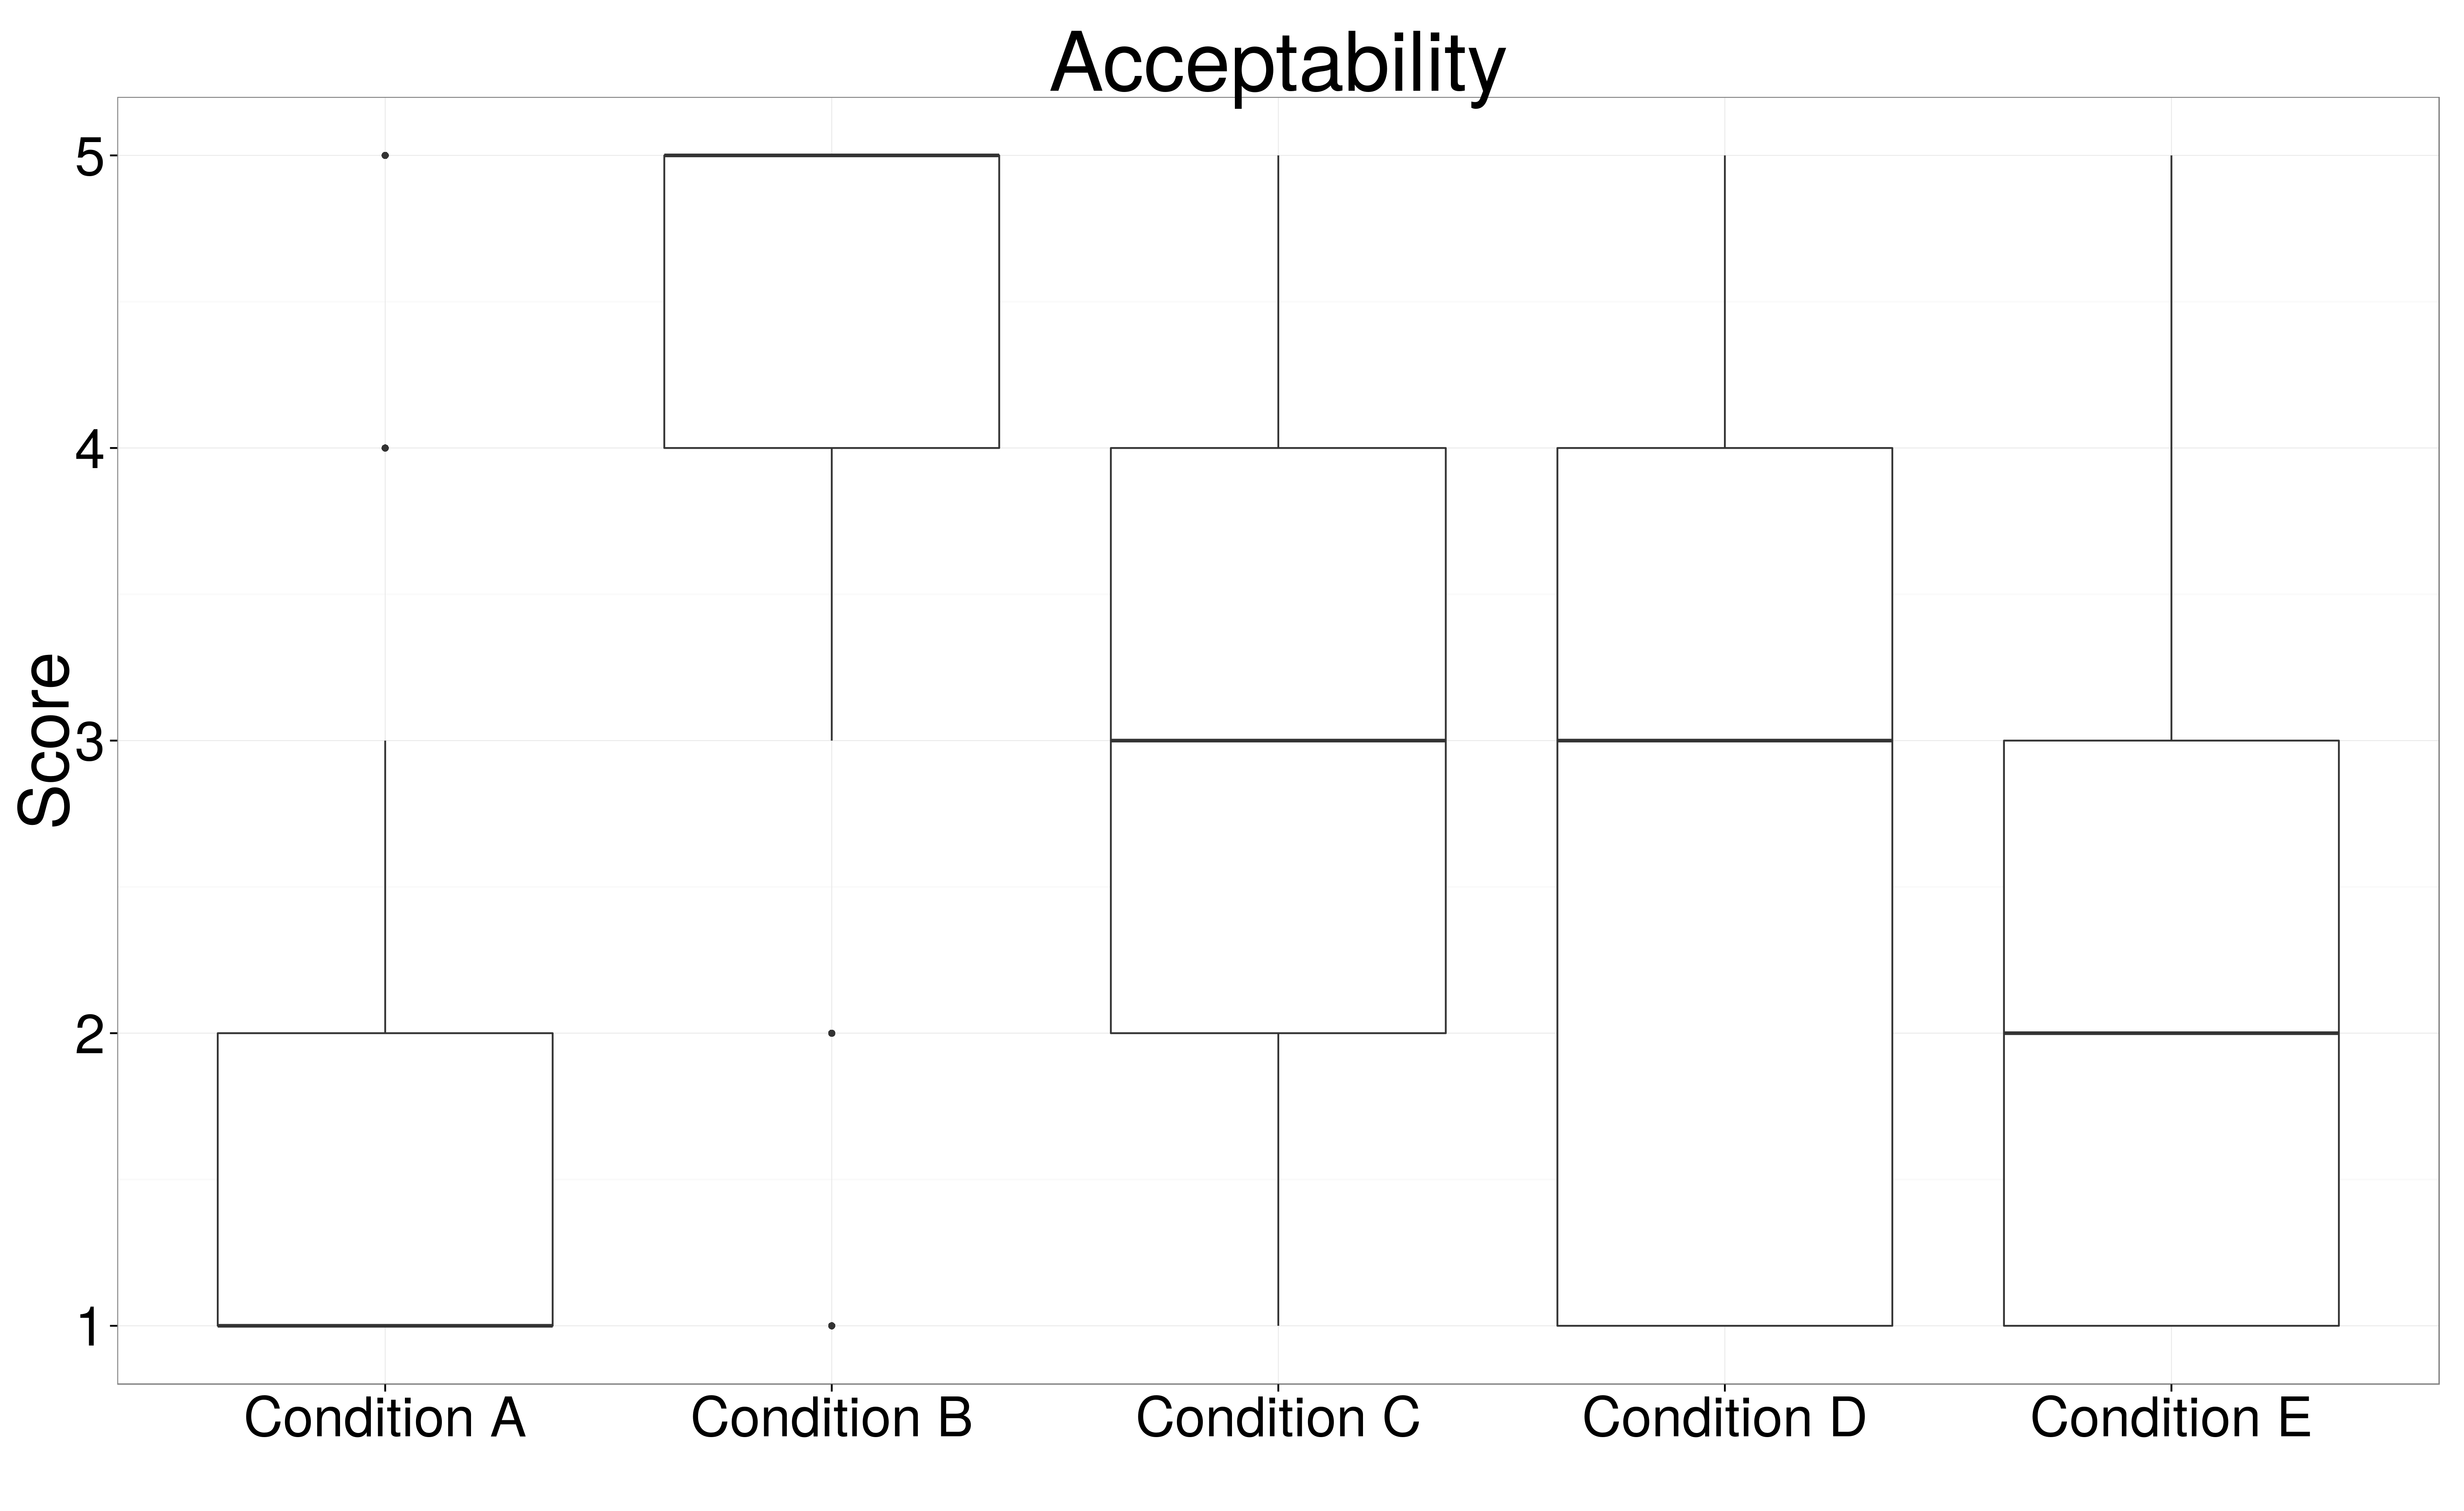
\includegraphics[scale=0.22]{figures/boxplot-exp1.png}
\caption{Results of Experiment 1}
\label{fig1_stat}
\end{figure}


The results of the experiment can be theoretically explained in the scalar approach to NR \citep{horn1973semantic,romoli2012soft,romoli2013scalar}. In the scalar theory of neg-raising  NR predicates (beside the assertion -- \REF{ex-25-a}) contribute the  excluded middle (EM) \isi{implicature} to the semantic composition \REF{ex-25-b}. And finally the   alternatives generated by the \isi{implicature} are exhaustified by \cnst{exh} -- \REF{ex-26}.

\ea \ea \label{ex-25-a} $\llbracket$NR$\rrbracket = \lambda p\lambda x.\square_x[p]$
\ex \label{ex-25-b} $\cnst{alt}(\llbracket$NR$\rrbracket)=\{\lambda p\lambda x.\square_x[p],\lambda p\lambda x.[\square_x[p] \vee \square_x[\neg p]]\}$
\z
\z

\ea \label{ex-26} $\cnst{exh}(\cnst{alt}(p))(p)(w) = p(w) \wedge \forall q \in \cnst{excl}(p,\cnst{alt}(p))[\neg q(w)]$
\z

\noindent I will illustrate the mechanics of the scalar theory of NR on an example item from Experiment 1: \REF{ex-27}. Formula in \REF{ex-28-a} shows the alternatives generated by the excluded middle \isi{implicature} from \REF{ex-25-b}: it is the negated \isi{at-issue meaning} ($\neg \textsc{want}_s[p]$) and the excluded middle part ($\neg(\textsc{want}_s[p] \vee \textsc{want}_s[\neg p])$). The excluded middle in this case formalizes the involvement of the subject \textit{s}: he either wants the proposition \textit{p}, or he wants the \isi{negation} of \textit{p} but he cannot be uninterested with respect to \textit{p}. The excluded middle for other classes of NR-predicates has an analogous meaning: opinionatedness for \textit{know}/\textit{believe}, clear intentions for \textit{plan}, etc. Compare the lack of such an excluded middle meaning in predicates of communication: a speaker can say \textit{p} or neg \textit{p} but he can be silent about \textit{p} as well. \REF{ex-28-b} then shows the exhaustification of the alternatives: the \isi{at-issue meaning} remains the same but the excluded alternative is negated -- the usual strenghtening of the sentence meaning via negating its alternatives. The \isi{at-issue meaning} and double negated excluded middle alternative then (via deductive reasoning) yield the semantic low scope of \isi{negation} in the embedded proposition. So, as a consequence of exhaustification of the NR predicate and its excluded middle \isi{implicature}, the \isi{negation} is of the NR predicate is interpreted as having low scope (semantically).

\ea\label{ex-27} `A new shepherd in Tatra mountains doesn't want even one sheep to be missing.'\\ $\neg \textsc{want}_s[p]$
\z

\ea \ea \label{ex-28-a}$\cnst{alt}(\neg \textsc{want}_s[p])=\{\neg \textsc{want}_s[p], \neg(\textsc{want}_s[p] \vee \textsc{want}_s[\neg p])\}$
\ex \label{ex-28-b}$\cnst{exh}(\neg \textsc{want}_s[p])=\neg \textsc{want}_s[p] \wedge \neg \neg(\textsc{want}_s[p] \vee \textsc{want}_s[\neg p]) \models \textsc{want}_s[\neg p]$
\z
\z

\noindent Let us recall that strong NPIs are licensed by anti-additive functions: functions which obey deMorgan's laws which naturally is true for \isi{negation}: a natural language example is presented in \REF{ex-29-a} and \REF{ex-29-b} where the \isi{entailment} is bidirectional and in propositional logic in \REF{ex-29-c} and \REF{ex-29-d} where the same meaning equivalence holds.

\ea \ea\label{ex-29-a} It didn't rain and it didn't snow.
\ex \label{ex-29-b} It didn't rain or snow.
\ex \label{ex-29-c} $\neg p \wedge \neg q$
\ex \label{ex-29-d} $\neg[p \vee q]$
\z
\z

\noindent In the case of NR predicates like \textit{want} in \REF{ex-30} the embedded clause qualifies as an anti-additive environment due to the NR-transfer of \isi{negation}: \REF{ex-30-a} is equivalent to \REF{ex-30-b} -- both require \textit{p} and \textit{q} being false in all possible worlds -- see \tabref{tab:table4_w1_w2} with an example of two possible worlds. In such a model both logical formulas in \REF{ex-30-c} and \REF{ex-30-d} are true.

\ea \label{ex-30}\ea \label{ex-30-a} Susan does not want to sleep and she does not want to dance.
\ex \label{ex-30-b} Susan does not want to sleep or dance.
\ex \label{ex-30-c} $\square \neg p \wedge \square \neg q \leftrightarrow$
\ex \label{ex-30-d} $\square \neg(p \vee q)$
\z
\z

\begin{table}
\begin{tabularx}{0.4\textwidth}{lXX}
\lsptoprule
world/proposition & $p$ & $q$\tabularnewline
\midrule
$w_1$ & 0 & 0\tabularnewline
$w_2$ & 0 & 0\tabularnewline
\lspbottomrule
\end{tabularx}
\caption{A fragment of possible worlds for \REF{ex-30}}
     \label{tab:table4_w1_w2}
\end{table}


\noindent But consider an example of non-NR predicates like \textit{say} in \REF{ex-31-a} and \REF{ex-31-b}. \REF{ex-31-b} does not follow from  \REF{ex-31-a} since non-NR predicates if negated allow only the high scope of \isi{negation} interpretation: \REF{ex-32-a} -- and such an interpretation is the following: it requires there to be at least some possible worlds where the propositions \textit{p} and \textit{q} are false. But \REF{ex-32-a} is stronger: it requires both propositions \textit{p} and \textit{q} to be false in all possible worlds. \REF{ex-32-a} would be true in a valuation of propositions across possible worlds in \tabref{tab:table5} but \REF{ex-32-b} would be false in such a model. In other words: non-NR predicates do not create anti-additive environment in their embedded clauses. And since strong NPIs need anti-additivity, they are unlicensed in the embedded clauses of non-NR predicates.

\ea \ea\label{ex-31-a} Susan didn't say that she will sleep and she didn't say that she will dance.
\ex \label{ex-31-b} Susan didn't say that she will sleep or dance.
\z
\z

\ea \ea\label{ex-32-a} $\neg \square p \wedge \neg \square q$ (true in the table)
\ex \label{ex-32-b}$\neg \square[p \vee q]$ (false in the table)
\z
\z

\begin{table}
\begin{tabularx}{0.4\textwidth}{lXX}
\lsptoprule
world/proposition & $p$ & $q$\tabularnewline
\midrule
$w_1$ & 0 & 1\tabularnewline
$w_2$ & 1 & 0\tabularnewline
\lspbottomrule

\end{tabularx}
\caption{A fragment of possible worlds for \REF{ex-31-a}/\REF{ex-31-b}}
     \label{tab:table5}
\end{table}


\noindent Returning now to the initial predictions: Experiment 1 confirmed the \isi{NPI} status of \textit{ani (jeden)} -- if \textit{ani (jeden)} were an n-word, the contrast between NR predicates (\textit{ani (jeden)} licensed) and non-NR predicates (\textit{ani jeden} not acceptable) would be unexplained since syntactic licensing should not be sensitive to semantic distinctions between anti-additive and non-anti-additive environments. So we can conclude this section with a first clear  experimental confirmation of classifying \textit{ani (jeden)} as a strong \isi{NPI}. Moreover it was established that anti-additivity is a necessary condition for licensing the strong \isi{NPI} \textit{ani (jeden)}. Experiment 1 itself did not establish contrast between strong NPIs (\textit{ani (jeden)}) and n-words but its results would be unexpected if \textit{ani (jeden)} were not a strong \isi{NPI}. Experiment 1 did not test intuitions for \textit{žádný}, the reason for that is the following one: \textit{žádný} is perceived by native \ili{Czech} native speakers to be grammatical only if it appears in a sentence with local \isi{negation} \REF{ex-24-b} type of sentences. So unlike in case of \textit{ani (jeden)} where the judgments are much more graded, there is no need to experimentally establish the acceptability of \textit{žádný}.

\begin{table}
\begin{tabularx}{0.6\textwidth}{lXX}
\lsptoprule
environment/status & NPIs & n-words\tabularnewline
\midrule
NR embedded & \ding{51} & \ding{55}\tabularnewline
non-NR embedded & \ding{55} & \ding{55}\tabularnewline
\lspbottomrule
\end{tabularx}
\caption{N-words vs. NPIs in Neg-raising environments}
     \label{table6}
\end{table}



\subsection{Fragment answers}\label{fragment-answers}

Another distinction mentioned already in criterion \ref{nwords-npi-crit} is the distinction between n-words and NPIs with respect to their ability to be fragmentary answers to questions. Roughly, n-words are good fragmentary answers, while NPIs are generally not acceptable as fragmentary answers. Similarly to the situation in NR contexts reported in the last section, the acceptability of \textit{ani (jeden)} as a fragmentary answer seems to be more varied than in case of n-words which are always good as fragment answers. I pre-experimentally noticed that especially in cases where the question supplies more context, the NPIs seem more acceptable, following the pattern in \REF{ex-32-5}. The fragment answers were tested in two expriments; first in Experiment 2 the fragment answers were tested against minimal context questions.

\ea \label{ex-32-5} \ea[]{ \gll Kdo byl dneska večer na náměstí?\\
who was today evening on square?\\
\glt `Who was today in the evening on the square?'}
\ex[?]{ \gll Ani jeden člověk.\\
\textsc{npi} one human\\
\glt `Not even one man.'}
\ex[]{\gll Kdo tu dneska byl?\\
who here today was\\
\glt `Who was here today?'}
\ex[???] {\gll Ani jeden člověk.\\
\textsc{npi} one human\\
\glt `Not even one man.'}
\z
\z


\noindent In Experiment 2 (details can be found in \citealt{docekaldotlacilsubber}), there was a negative interaction of \textit{ani} and \isi{ellipsis} in non-negative questions like \REF{ex-33}. In other words, as expected n-words were judged by speakers as better fragmentary answers than NPIs. The statistical outcome is visualized in \figref{fig:exp2} -- the relevant condition is \textsc{ellipsis}  and blue bar for n-words, red for NPIs.

\ea[]{\label{ex-33}\gll Kdo odešel z hospody?\\
who left from pub?\\
\glt `Who left the pub?'}
\ea[]{\gll  Žádný student.\\
\textsc{n-adj} student\\
\glt `No student.'}
\ex[??]{\gll Ani jeden student.\\
\textsc{npi} one student\\
\glt `Not even one student.'}
\z
\z

\begin{figure}
\centering
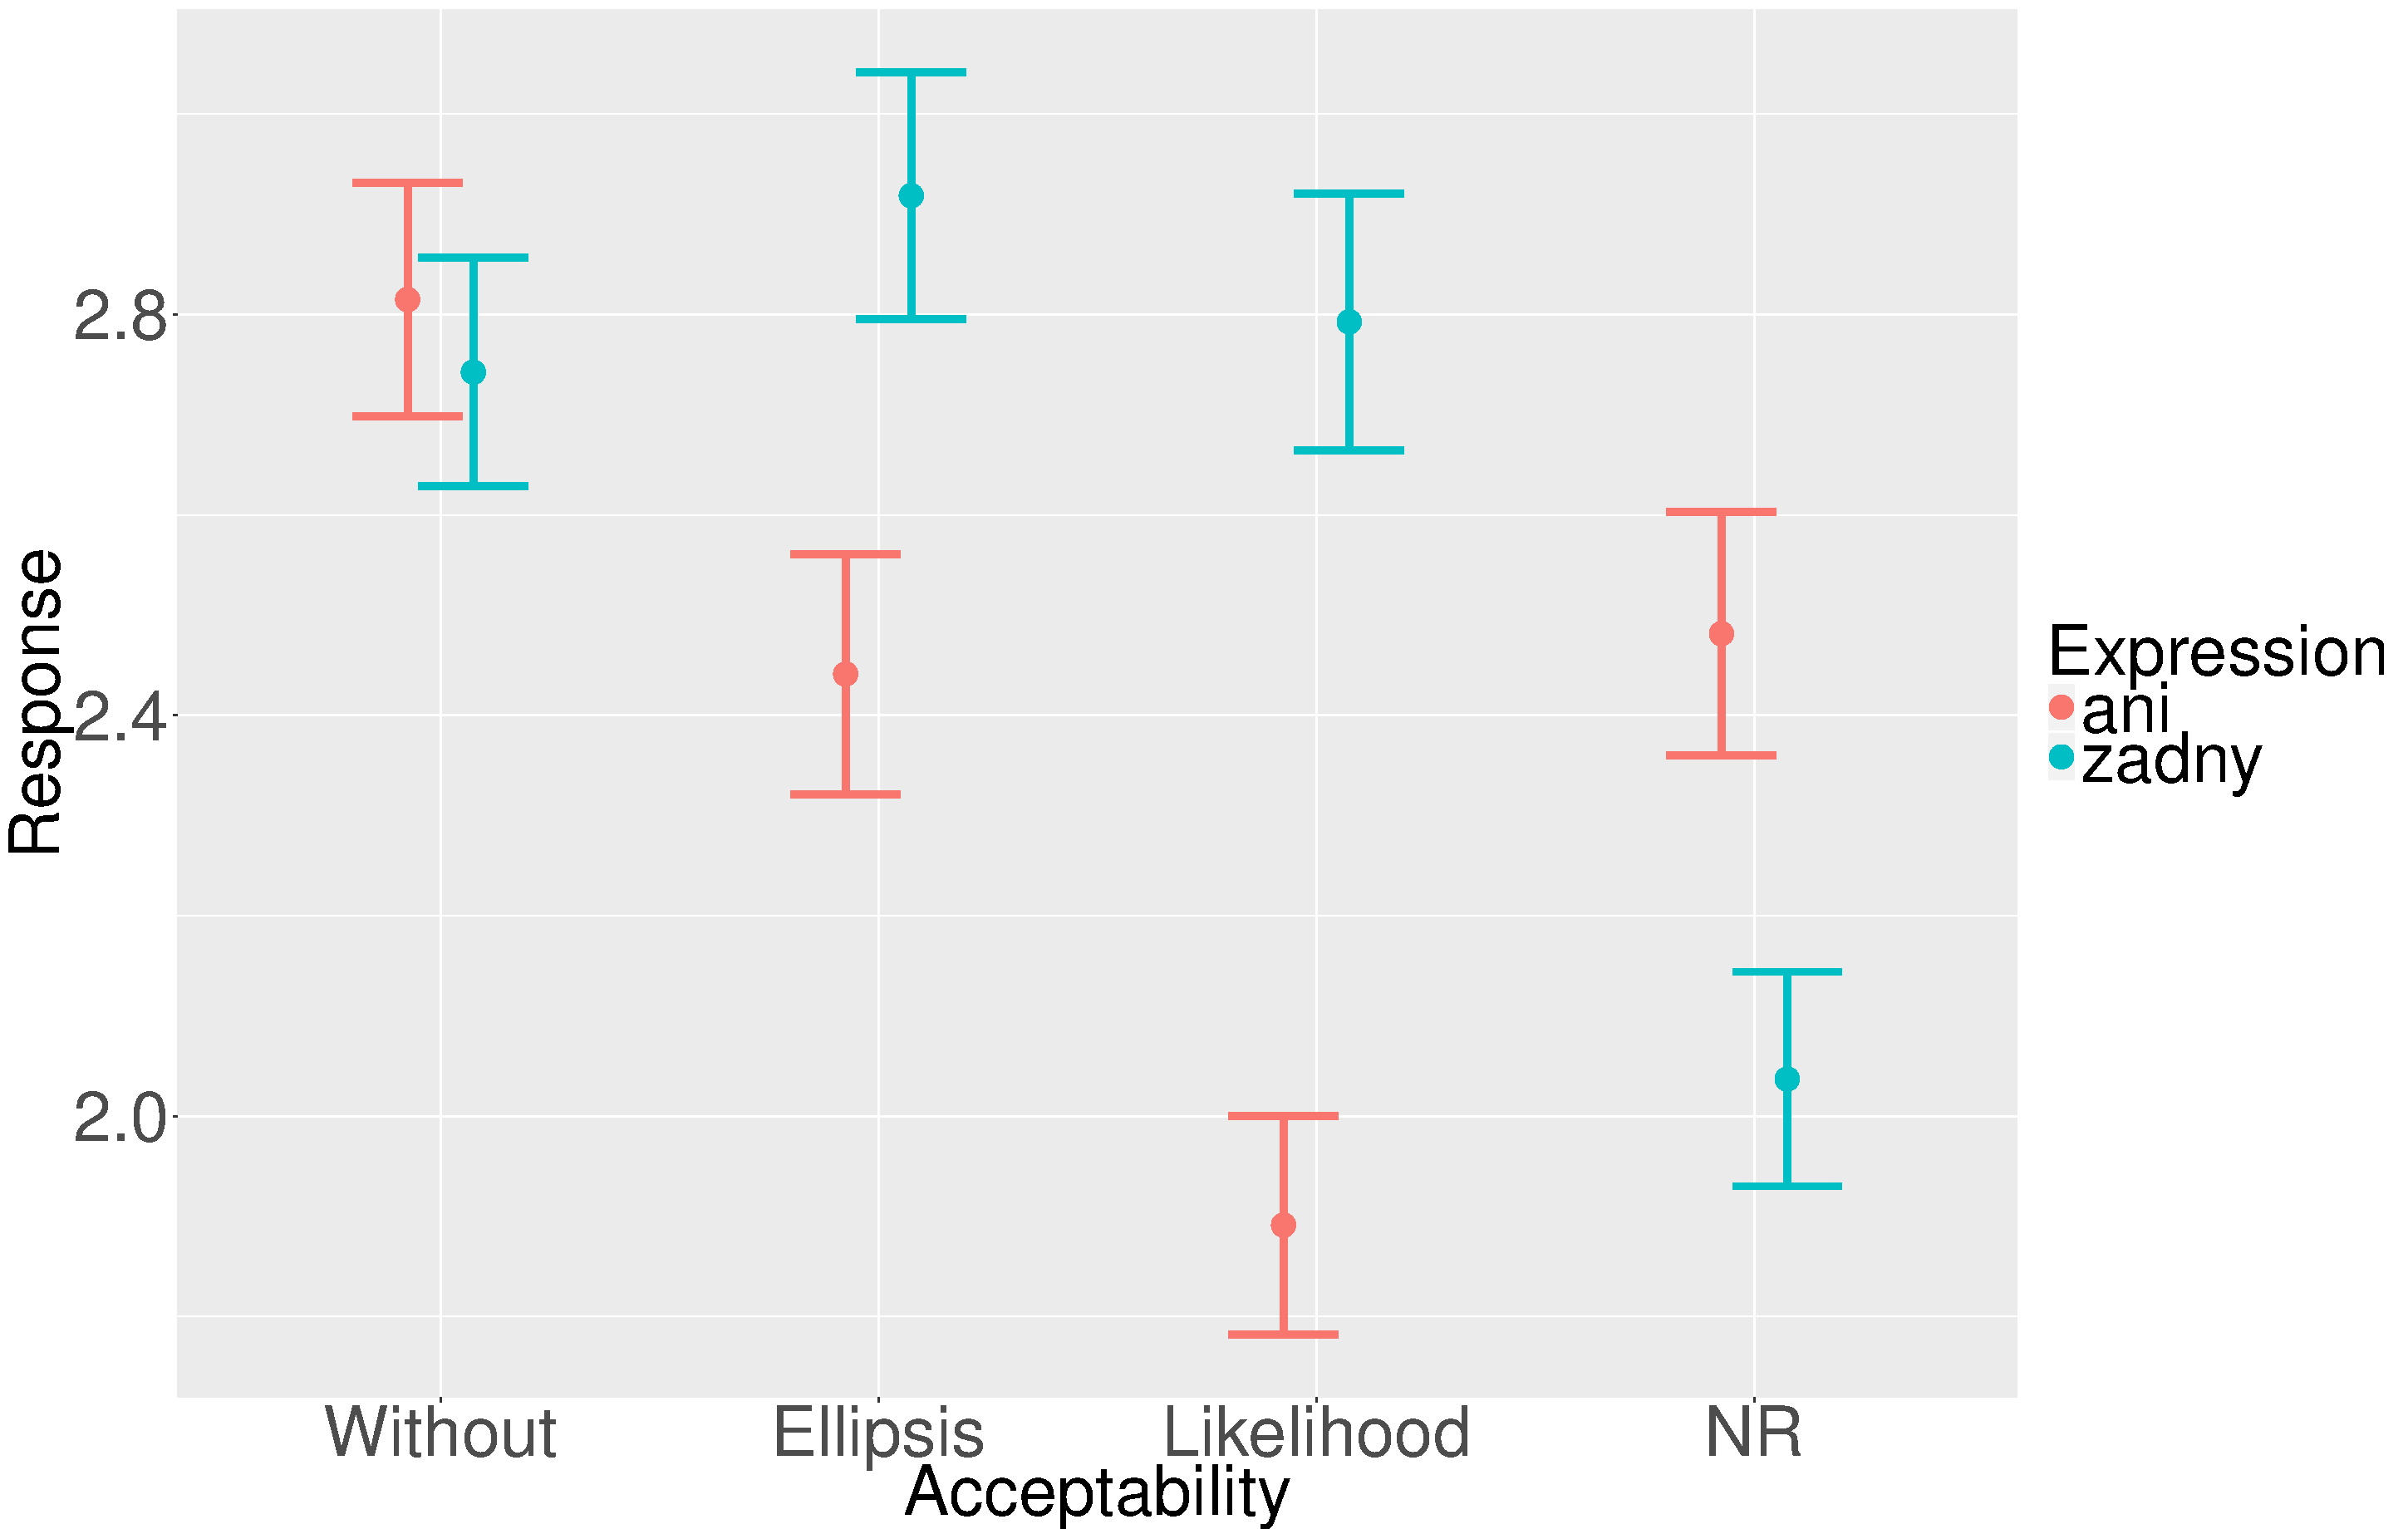
\includegraphics[scale=0.25]{figures/mean-sum.png}
\caption{Results of Experiment 2}\label{fig:exp2}
\end{figure}

\noindent The theoretical explanation of this known difference is usually provided via a possible reconstruction of n-words and unavailability of reconstruction for NPIs. Because NPIs are usually not able to reconstruct under a possible licensor in their scope \citep{de1998licensing} like in the following example where \isi{NPI} \textit{any} student in the cleft cannot reconstruct to its base \isi{object position} under the \isi{quantifier} \textit{no professor} which would license it.%
\footnote{Again the ban on \isi{NPI} reconstruction can be side-stepped with a carefully constructed example as the following sentence from \cite[p.17]{uribe1994interface} shows: \textit{A doctor who knew anything about acupuncture was not available}. It seems though that in such cases it is the whole subject NP (containing the \isi{NPI}) reconstruction which saves grammaticality of \isi{NPI} and this type of construction seems to be highly restricted. Nevertheless thanks to an anonymous reviewer for pointing this out.}

\ea *It is any student that no professor likes.
\z

\noindent We further elaborated the fragment answer distinction in Experiment 3 (details can be found in \citealt{docekaldotlacilsubber}) where we provided more contextual informations like in the example item \REF{ex-35}. In this experiment the correlation disappeared: see \figref{fig:exp3} -- conditions \textsc{FragNPI} vs. \textsc{FragNword} with no difference in acceptability.

\ea \label{ex-35} \gll Koho vyhodil profesor Palný včera ze zkoušky?\\
whom fired prof Palný yesterday from exam?\\
\glt `Who was fired by prof Palný during yesterday's exam?'
\ea \gll Žádného studenta.\\
\textsc{n-adj} student\\
\glt `No student.'
\ex \gll Ani jednoho studenta.\\
\textsc{npi} one student\\
\glt `Not even one student.'
\z
\z

\begin{figure}
\centering
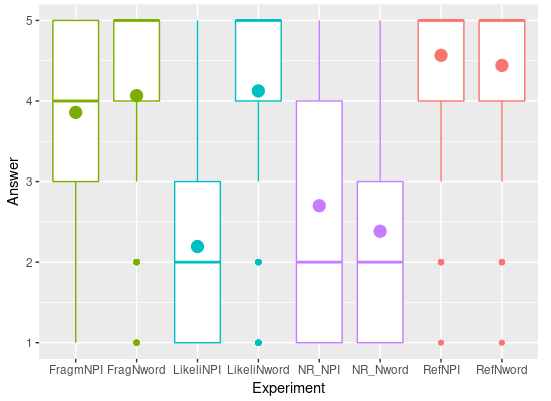
\includegraphics[scale=0.8]{figures/Rplot04.png}
\caption{Results of Experiment 3}\label{fig:exp3}
\end{figure}

\noindent The ability of n-words to appear as fragmentary answers is usually taken as the standard distinction of n-words against NPIs. But in a recent paper  \cite{fualuaus2016fragment} observe a strikingly related phenomen: the authors claim (based on data from many \isi{strict neg-concord} languages) that in \isi{strict neg-concord} languages n-word answers to negative questions can have (surprisingly) a Double Negation (DN) reading. This observation goes against the n-words vs.~NPIs criterion as it falsifies the meaning part of it: n-words and (reconstructed) \isi{negation} yield only one semantic \isi{negation}. I checked \citeposst{fualuaus2016fragment} claims with 10 native speakers of \ili{Czech} and they seem to be valid -- see example \REF{ex-36}: there seems to be even a preference (8/10) for the DN reading -- \REF{ex-36-a} but the \isi{negative concord} reading \REF{ex-36-b} is considered to be possible (for 2 out of 10 speakers).

\ea\label{ex-36} \gll Kdo nepřečetl žádný článek?\\
who neg.read \textsc{n-adj} article\\
\glt `Who didn't read any article?'
\ea\label{ex-36-a} Nikdo.\\
Nobody. (None of us read a single one.) NC (2/10): $\neg \exists x,y[\textsc{person}(x) \wedge \textsc{article}(y) \wedge \textsc{read}(x,y)]$\\${}\equiv\forall x[\textsc{person}(x) \rightarrow \neg \exists y[\textsc{article}(y) \wedge \textsc{read}(x,y)]]$
\ex\label{ex-36-b} Nikdo.\\
Nobody. (Each of us read an article) DN (8/10):  $\neg \exists x[\textsc{person}(x) \wedge  \textsc{article}(y) \wedge \neg \textsc{read}(x,y)]$\\${}\equiv\forall x[\textsc{person}(x) \rightarrow \exists y[\textsc{article}(y) \wedge \textsc{read}(x,y)]]$
\z
\z

\noindent \cite{fualuaus2016fragment} solve the availability of DN reading of n-words via postulating another (focus-related) position for covert \isi{negation} (\isi{CN}): in the \isi{left periphery} of a clause as in the tree in \figref{ex-37}. The position is according to \cite{fualuaus2016fragment} licensed via n-word movement to the left peripheral position above TP. A \isi{negation} in the \isi{left periphery} is a second \isi{negation} in a sentence, next to the reconstructed \isi{negation} from the question (surface \isi{negation}, SN). So the first \isi{negation} in \REF{ex-36-b} is the interpretation of covert \isi{negation}, the second one of the \isi{verbal negation}. If we follow \cite{fualuaus2016fragment}, we can explain the puzzling disappearance of contrast between n-words and NPIs (Experiment 3) as a consequence of the covert \isi{negation} -- if such a \isi{negation} appears in a clause, the NPIs are licensed because they do not need to reconstruct under the scope of \isi{verbal negation} and then the contrast between n-words and NPIs disappears.

\begin{figure}
% $\Tree[[.\isi{CN} ] [[.FOC n-word ][.TP [] [.NegP [. SN ] [.VP [.V ] n-word ]]]]]$
\begin{forest}for tree={s sep=10mm,inner sep=0, l=0}
    [,s sep=15mm
        [\isi{CN}]
        [,s sep=5mm
            [FOC
                [n-word]
            ]
            [TP
                [,phantom]
                [NegP
                    [SN]
                    [VP
                        [V]
                        [n-word]
                    ]
                ]
            ]
        ]
    ]
\end{forest}
\caption{Covert negation, syntax}\label{ex-37}
\end{figure}

\noindent There are many questions raised by postulating such covert \isi{negation}, especially with respect to possible over-generation -- at the end n-words in \isi{strict negative concord} languages cannot appear in sentences without \isi{negation} but postulating covert \isi{negation} leaves this robust observation unexplained. \cite{fualuaus2016fragment} try to resolve such problems by restricting the covert \isi{negation} only to controllable set of cases, all somehow related to \isi{focus} movement of n-words to the \isi{left periphery}. I tried to verify their claims and conducted a small survey again with the same 10 speakers of \ili{Czech} and it seems that \citeauthor{fualuaus2016fragment}'s general idea is confirmed with an interesting twist. Let us start with a basic case -- \REF{ex-38} is interpreted only with NC reading as is visible from the ranking in \REF{ex-38-a} and \REF{ex-38-b} -- a double \isi{negation reading} is simply non-existent.

\ea\label{ex-38} \gll Nikdo ničemu nevěří.\\
\textsc{n-person} \textsc{n-thing} \textsc{neg}.believes\\
\glt `Nobody believes anything.'
\ea[]{\label{ex-38-a} NC: $\forall x[\textsc{person}(x) \rightarrow \neg \exists y[\textsc{entity}(y) \wedge \textsc{believe}(x,y)]]$}
\ex[*]{\label{ex-38-b} DN: $\forall x[\textsc{person}(x) \rightarrow \exists y[\textsc{entity}(y) \wedge \textsc{believe}(x,y)]]$}
\z
\z

\noindent But in case of information structure manipulation like in \REF{ex-39}, which is even an \isi{affirmative sentence}, the double \isi{negation reading} surprisingly emerges. A similar pattern is observed in \REF{ex-40}. The sentences moreover seem to have the double \isi{negation reading} only. This confirms \citeauthor{fualuaus2016fragment}'s hypothesis about \isi{focus} position of the \isi{CN}: example \REF{ex-38}, where there is no object movement to the \isi{left periphery} (unlike in \REF{ex-39} and \REF{ex-40}), has only the expected NC reading. In this article it is not possible to explore more details of this interesting appearance of double \isi{negation reading} in a \isi{negative concord} language like \ili{Czech} but more importantly: it seems to be reasonable to postulate another position for \isi{negation} in the \isi{left periphery} of a clause, such a position (because it is somehow licensed via \isi{focus}) can then blur the picture of the fragmentary answer criterion and the fluctuation of acceptability of NPIs as fragmentary answers observed in Experiment 3 is no longer a mystery, context manipulation can lead to a \isi{focus} related \isi{CN} licensing of even strong NPIs as fragment answers.

\ea\label{ex-39}  \gll V nic nikdo nevěří.\\
in \textsc{n-thing} \textsc{n-person} believes\\
\glt `Nobody believes in anything.'
\ea[*]{ NC (0/10): $\forall x[\textsc{person}(x) \rightarrow \neg \exists y[\textsc{entity}(y) \wedge \textsc{believe}(x,y)]]$}
\ex[]{  DN (10/10): $\forall x[\textsc{person}(x) \rightarrow \exists y[\textsc{entity}(y) \wedge \textsc{believe}(x,y)]]$}
\z
\z

\ea\label{ex-40} \gll Nic při té zkoušce nikdo nenapsal.\\
\textsc{n-thing} at the exam \textsc{n-person} \textsc{neg}.wrote\\
\glt `Nobody wrote anything during the exam.'
\ea[*]{NC (0/10): $\forall x[\textsc{person}(x) \rightarrow \neg \exists y[\textsc{entity}(y) \wedge \textsc{write}(x,y)]]$}
\ex[]{ DN (10/10): $\forall x[\textsc{person}(x) \rightarrow \exists y[\textsc{entity}(y) \wedge \textsc{write}(x,y)]]$}
\z
\z

\noindent Summary of this section: there seems to be some evidence for classifying \textit{ani} as an \isi{NPI} and \textit{žádný} as an n-word which stems from the fragment answer experiments. When the results diverge from the expected dichotomy, there seems to be a reasonable explanation via postulation of a second covert \isi{negation} in the sentence.

\subsection{Likelihood scenarios}\label{likelihood-scenarios}

The last environment discussed in this article concerns the semantic properties of sentences where n-words vs. NPIs occur. The straightforward predictions are the following:

\begin{enumerate}
  \def\labelenumi{\arabic{enumi})}
%   \tightlist
  \item
    n-words (licensed in syntax) should not be sensitive to logical properties of
    their environment (they require just sentential/\isi{verbal negation})
  \item
    NPIs are licensed in semantics and by definition are dependent on semantic properties like DE, anti-additivity, etc.
\end{enumerate}

\noindent I will pursue the line of distinguishing NPIs from n-words via the \isi{NPI} sensitivity to monotonicity and likelihood. And I will base my reasoning on a very influential theory of \isi{NPI} licensing, the so called simple
  \textit{even} hypothesis of \isi{NPI} licensing (\citealt{heim1984note,krifka1995semantics,crnivc2014against} -- I will call the theory Heim/Crnič theory further). The theory describes NPIs using the following three ingredients:

  \begin{itemize}
%   \tightlist
  \item
    NPIs associate with covert \textit{even} -- the formalization can be via a formal [$even$] feature carried by the NPIs, etc.
  \item
    NPIs (like focused element) generate sets of possible alternatives;
  \item
    covert \textit{even} associates with the alternatives and generates
    \isi{presupposition} of its prejacent being the least probable member of
    the set of alternatives (entailing all the alternatives) -- in case of association with \textit{even} (some authors suggest different covert licensors of NPIs too);
  \end{itemize}

\noindent The immediate predictions of the Heim/Crnič theory is that NPIs should be sensitive to probability and entailing properties. The first and the second one are logically related: a proposition \textit{p} cannot be more likely than a proposition \textit{q}, if \textit{p} entails \textit{q}: intuitive illustration -- \textit{p} being \textit{Rambo killed 100 enemies}, \textit{q} being \textit{Rambo killed 99 enemies}, \textit{p} entails \textit{q} and \textit{p} is less likely than \textit{q}; \textit{q} does not entail \textit{p} and is more likely than \textit{q} -- see \cite{crnic2011getting} for details of relating entailing and likelihood. The theoretical intricacies away, the prediction that NPIs should be sensitive to logical properties like entailing or probability while n-word not is uncontroversial, see \tabref{tab:log_properties} for a visualization of these predictions.

\begin{table}
\begin{tabularx}{0.55\textwidth}{ll}
\lsptoprule
property/item & \isi{entailment}/probability\tabularnewline
\midrule
n-words & \ding{55}\tabularnewline
NPIs & \ding{51}\tabularnewline
\lspbottomrule
\end{tabularx}
\caption{N-words vs. NPIs in probability manipulated environments }
     \label{tab:log_properties}
\end{table}

And exactly this prediction was tested in Experiment 2 and Experiment 3. In both we found a strong correlation of \textit{ani} and probability. As a side note: a corpus survey (the biggest national \ili{Czech} corpus,  \cite{Krenetal2015}) confirms the likelihood sensitivity of \textit{ani} -- a prototypical example in \REF{ex-41} shows that \textit{ani} usually associates with weak scalar items (\textit{ani jeden} is the second most frequent collocation, the first one another minimizer \textit{ani slovo} `not a single word'). which via scalar reasoning entails all other scalar alternatives ($\neg \exists X[\textsc{customer}(X) \wedge \#X=1 \wedge \textsc{enter}(X)] \rightarrow \neg \exists X[\textsc{customer}(X) \wedge \#X>1 \wedge \textsc{enter}(X)]$). And due to this \isi{entailment} the sentence with \textit{ani} and a weak element associated with \textit{ani} is the least probable (entailing all other alternatives).

\ea\label{ex-41} \gll tento nyní úspěšný podnikatel {[}\ldots{}{]} v prvním měsíci neměl \minsp{[} ani jednoho zákazníka]\\
this now succesfull businessman {} in first month \textsc{neg}.had {} \textsc{npi} one customer {}\\
\glt `This currently succesfull businessman did not have even one customer in the first month.'
\z

\noindent\sloppy In Experiment 2 the acceptability of \textit{ani} with strong scalar items was tested -- example item in \REF{ex-42} where the scale of catholic hierarchy is most probably $\langle priest, bishop, cardinal\rangle$ -- \textit{cardinal} being high \isi{scalar item} in any case. The scale entails contextual (not proper formal logical) \isi{entailment} due to the facts of world we know the following implicational hierarchy: $\exists x[\textsc{become cardinal}(x)$ $\rightarrow \textsc{become bishop}(x) \rightarrow \textsc{become priest}(x)]$ and its reversal as invalid: $\exists x$ $[\textsc{become priest}(x) \not\rightarrow$ $\textsc{become bishop}(x) \not\rightarrow \textsc{become cardinal}(x)]$. To acquire the grade of cardinal entails acquiring (ceteris paribus) acquiring all lower ranks of catholic hierarchy but not the other way round. The \isi{scalar item} \textit{cardinal} is the strongest (in the ad hoc scale), it entails all other items in the scale and is consequently least likely (which fits the natural intuitions). If \textit{ani} prefers weak scalar items, it should be degraded with strong items, while n-words (as they are not picky about semantic environments) should be more acceptable.

\ea \label{ex-42} {[{\ldots{}}]} \gll nestal se \{\hspace{-2pt} ani / žádným\} kardinálem\\
\textsc{neg.}became \textsc{se} {} \textsc{npi} {} \textsc{n-adj} cardinal\\
\glt `He didn't become even a cardinal.'
\z

\noindent And we found out that people overall preferred \textit{žádný} (n-word) with strong scalar items. The reason is that n-words do not have semantic requirements unlike NPIs: \textit{ani} prefers weak scalar items. The statistical results of Experiment 2 are in  \figref{fig:exp2}, the pertinent condition \textsc{likelihood}: \textit{ani} (red) had mean acceptability very much below the n-word's mean acceptability (blue) (around 2.8 for n-words).

Experiment 3 was partially an elaboration of Experiment 2 -- while Experiment 2 used an acceptability task, in Experiment 3 the truth value judgment task was used in case of testing likelihood properties of \textit{ani}. An example item is in \REF{ex-43}. Again it was tested how much worse is the acceptability of strong scalar items with \textit{ani}. In this scenario the scale is $\langle \text{PhD}, \text{MA}, \text{BA}\rangle$: here the scale is contextually based on the likelihood of passing the exam (if the scale were based simply on academic hierarchy, as in the acceptability testing in \REF{ex-42}, it would be $\langle \text{PhD}, \text{MA}, \text{BA}\rangle$ but in \REF{ex-43} the scale is reversed as passing the exam is prototypically negatively correlated with the academic rank). The scale is (due to the context) again based on contextual \isi{entailment}: $\forall x[\textsc{BA}(x) \rightarrow  \textsc{pass}(x)] \rightarrow [\forall x[\textsc{MA}(x) \rightarrow \textsc{pass}(x)] \rightarrow \forall x[\textsc{PhD}(x) \rightarrow \textsc{pass}(x)]]$. Therefore \textit{ani} associates again with the strongest \isi{scalar item} (in the positive version of a tested sentence entailing all its scalar alternatives). And as the statistical summary in \figref{fig:exp3} shows (the relevant condition \textsc{Likeli\_NPI} s. \textsc{Likeli\_Nword} -- blue color), speakers again preferred n-words to \textit{ani} NPIs.  This again follows from \textit{ani}'s semantic requirements (it associates with weak items which in negative contexts become least likely among alternative scalar items)  vs. n-words which do not have any semantic sensitivity and are therefore more acceptable than \textit{ani}.

\eanoraggedright\label{ex-43} Scenario: prof. Novák yesterday examined an easy course which BA, MA~and PhD~students attend. PhD~students pass the exam always, MA~in most cases but BA only rarely.
\gll Včerejší zkoušku u prof. Nováka nesložili \{\hspace{-2pt} ani / žádní\} bakaláři.\\
yesterday exam at prof. Novák \textsc{neg}.passed {} \textsc{npi} {} \textsc{n-adj} BA-students\\
\glt `No bachelors passed the yesterday's exam by prof. Novák.'
\z


\noindent Empirically both experiments strongly support the classification of \textit{ani} as an \isi{NPI} which associates with weak scalar items and \textit{žádný} as an n-word licensed in the syntax (and consequently without any particular semantic sensitivity).

\begin{table}
\begin{tabularx}{0.55\textwidth}{ll}
\lsptoprule
property/item & probability/\isi{entailment}\tabularnewline
\midrule
\textit{žádný} & \ding{55}\tabularnewline
\textit{ani} & \ding{51}\tabularnewline
\lspbottomrule
\end{tabularx}
\caption{\textit{Ani} vs. \textit{žádný} in probability manipulated environments }
     \label{tab:table8}
\end{table}


The theoretical explanation of \textit{ani} being an \isi{NPI} which obligatorily selects weak scalar items can be the following. The first thing to note is that the facts observed in the experiments are only a piece of a bigger pattern where \textit{ani} competes in some environments with another scalar particle \textit{i} `even'. In a recent experiment \citep{docekalsafratovaoli} it was confirmed that \textit{i} obligatorily selects strong scalar items, while \textit{ani} weak items. Illustrated on a data pattern close to the catholic hierarchy from Experiment 2 \ili{Czech} native speakers are prone to the following judgments (where * should be understood as total unacceptability in experiments, ?? as in-between-acceptability and $\checkmark$ as nearly total acceptability -- statistic noise away -- but of course only in case the judgments are related to the set up scale, catholic hierarchy in \REF{ex-44}.

\ea\label{ex-44} \ea \textit{Upward entailing contexts:}
\ea \gll Petr se nakonec stal \{\ding{51}\hspace{-2pt} i kardinálem / ??\hspace{-2pt} i knězem\}.\\
Petr \textsc{se} at-end became {} even cardinal {} {} even priest\\
\glt `Petr in the end became \{ even a cardinal / even a priest \}.'
\newpage
\ex \gll Petr se nakonec stal \{*\hspace{-2pt} ani kardinálem / *\hspace{-2pt} ani knězem\}.\\
Petr \textsc{se} at-the-end became  {} not.even  cardinal {} {} not.even priest.\\
\glt `Petr in the end didn't become even a cardinal.'
\z
\ex \textit{Downward entailing, non anti-additive contexts:}
\ea \gll Jestli se Petr stal \{\ding{51}\hspace{-2pt} i kardinálem / ??\hspace{-2pt} i knězem\}, tak\ldots\\
If \textsc{se} Petr became {} even cardinal {} {} even priest then\\
\glt `If Peter became even a cardinal, then \ldots'
\ex\gll  Jestli se Petr stal *\hspace{-2pt} ani kardinálem, tak \ldots\\
If \textsc{se} Petr became {} not.even cardinal, then\\
\glt `If Peter didn't become even a cardinal, then \ldots'
\z
\ex  \textit{Downward entailing, anti-additive contexts:}
\ea  \gll Petr se nakonec nestal \{*\hspace{-2pt} i kardinálem / *\hspace{-2pt} i knězem\}.\\
Petr \textsc{se} at-the-end \textsc{neg}.become  {} even cardinal {} {} even priest\\
\glt `Petr didn't become even a cardinal at the end.'
\ex  \gll Petr se nakonec nestal \{??\hspace{-2pt} ani kardinálem /\hspace{1.2cm} \ding{51}\hspace{-2pt} ani knězem\}.\\
Petr \textsc{se} at-the-end \textsc{neg}.become {} not.even cardinal {} {} not.even priest\\
\glt `Petr didn't become even a cardinal at the end.'
\z
\z
\z

\noindent The pattern we observe is the following: \textit{i} in upward entailing contexts and downward entailing contexts prefers strong elements on a scale but it is unacceptable with weak or strong scalar items in anti-additive contexts; \textit{ani} prefers weak scalar items in anti-additive contexts but it is unacceptable in upward entailing contexts with both weak and strong scalar items (and in simple DE contexts). Such a pattern is explainable (following the logic of argumentation in \citealt{crnic2011getting}) as \textit{i} and \textit{ani} spelling out the following features:

\ea \ea \textit{i} {\ldots} [\textsc{even}]
\ex  \textit{ani} {\ldots} [\textsc{even},\textsc{aa}]
\z
\z

\noindent The feature [\textsc{even}] requires the association with covert \textit{even} defined below in \REF{ex-46} following \cite{crnivc2014against} among many others. The feature [\textsc{aa}] requires the item to occur in an anti-additive environment. The items form a scale in \REF{ex-47} and compete for insertion via the usual Maximize \isi{presupposition} principle which requires the speaker to make her contribution presupposing as much as possible (for the original formulation see \citealt{heim1991articles}).

\ea\label{ex-46} $\llbracket$even$\rrbracket^w (C)(p)$ is defined only if
$\forall q \in C[q \neq p \rightarrow q >_{\textsc{likely}} p]$
\z

\ea\label{ex-47} $\langle i,ani\rangle$
\z

\noindent The observed distribution of \textit{i}/\textit{ani} and their strong/weak association is explainable as follows:

\begin{enumerate}
	\item Upward entailing environments: \textit{i} is licit but only with strong scalar items as then the \textit{even} \isi{presupposition} is satisfied, \textit{ani} cannot be inserted as UE environments clash with \textit{ani} [\textsc{aa}] feature.
	\item Downward entailing environments: \textit{i} is licit with \textit{even} scoping below the DE operator:  {[} $\rightarrow$ {[}{[}even C{]} antecedent \ldots{} \textit{i} \ldots ] consequent ], \textit{ani} cannot be used due to the [\textsc{aa}] feature requirement.
	\item Anti-additive environments: \textit{i} cannot be inserted because Maximize Presupposition dictates the insertion of the most specific item (\textit{ani} in this case), \textit{ani} associates with weak scalar items: the scope [even C] [$\neg$ \ldots  \textit{ani} \ldots].
	\item The association of \textit{i}/\textit{ani} with 'wrong' scalar items is perceived as bad (??) but not totally ungrammatical -- weak \isi{scalar item} for \textit{i} in upward entailing contexts and strong scalar items for \textit{ani} in anti-additive environments.
\end{enumerate}

\noindent The last point seems to point to the existence of possible reversed scoping: [even C][$\rightarrow$ [antecedent \ldots \textit{i} \ldots] consequent ] for \textit{i} and  [$\neg$ [even C] \ldots \textit{ani} \ldots] for \textit{ani} which would explain their allowed (even if not preferred) 'crossed' association. But as it was confirmed by Experiment 2 and Experiment 3 \textit{ani} associates with weak items, while \textit{i} with strong scalar items (see \citealt{docekalsafratovaoli} for details) by default. This default scope exchange of \textit{i}/\textit{ani} which happens exactly in anti-additive contexts (\textit{i} prefers strong elements, \textit{ani} weak elements but only in the scope of \isi{negation} -- \isi{negation} being the anti-additive licensor in 99\%) reveals their unified semantics where the flip-flop is a consequence of \isi{entailment}/likelihood reversal caused by the \isi{negation}. The only difference between \textit{i} and \textit{ani} is the formal feature [\textsc{aa}] which formalizes the morphological incorporation of \isi{negation} into \textit{ani}.  It would be possible to encode the scope differences via different features ([\textsc{solo}] of \citealt{crnic2011getting} for the weak elements) but such a move would miss the nice competition pattern which emerged from the data: namely \textit{i} is in principle expected in anti-additive environments but cannot be inserted as a consequence of \textit{ani} being more specific ([\textsc{even,aa}]).

Summary of this section: \textit{ani (jeden)} `not even (one)' behaves like a strong \isi{NPI} -- this behavior was confirmed by Experiment 2 and Experiment 3 where association with strong scalar items was sanctioned (against relatively acceptable n-words modifying strong scalar items). Furthermore, \textit{ani} competes with \textit{i} -- the former prefers strong scalar items which was experimentally confirmed too. The association with weak scalar items and competition with \textit{i} would be unexpected if \textit{ani} were n-word.

\subsection{Summary}\label{summary}

Let us end this article by answering the question asked at the beginning: do  n-words and strong NPIs co-exist in natural language? And if yes (in some languages like \ili{English} they do co-exist for sure), does this distinction hold even in \isi{strict neg-concord} languages where the boundary between strong NPIs and n-words is even more subtle? The experiments, their results and their theoretical interpretation described in this article bring very strong support of the existence of both classes of negatively dependent expressions even in a \isi{strict neg-concord} language like \ili{Czech}. This result allows us to maintain the standard assumptions concerning n-words (they are licensed syntactically) and   NPIs (they are licensed in semantics/pragmatics). More importantly, the data patterns of \ili{Czech} NPIs seem to strongly favor the \isi{NPI} theories which base their licensing on concepts like  anti-additivity and likelihood (\citealt{zwarts1998three} in the first case, \citealt{heim1984note} and \citealt{crnivc2014against} in the second). Another issue touched in this article is unreliability of our intuitions: it seems that distinguishing between n-words and strong NPIs has to be based on such subtle data which can only be obtained by experimental methods. The subtlety of judgments can explain differing stances on this distinction in the previous literature where such opposing views as: n-words are a subclass of NPIs (\citealt{ladusaw1992expressing}, \citealt{fualuaus2016fragment} a.o.) versus n-words are a separate class (\citealt{zeijlstra2008negative} and \citealt{giannakidou2017landscape} a.o.) were maintained. There is another pertinent question raised by the data: do all speakers agree with respect to the distinction between n-words and strong NPIs? And if no, is there a real dialectal variation or at least some correlation? The results of the experiments in fact bear direct evidence on this fascinating question  but the space of this article is alas filled completely.

\section*{Abbreviations}

\begin{tabularx}{.5\textwidth}{@{}lX@{}}
\textsc{n-person}&{n-word for persons}\\
\textsc{n-thing}&n-word for things\\
\textsc{neg}&negation\\
\textsc{npi}&negative polarity item\\
\textsc{sbjv}&subjunctive\\
\textsc{de}&{downward entailing}\\
\textsc{pl}&{plural number}\\
\end{tabularx}%
\begin{tabularx}{.5\textwidth}{@{}lX@{}}
\textsc{sg}&{singular number}\\
\textsc{comp}&complementizer\\
\textsc{aux}&{auxiliary verb}\\
\textsc{n-adj}&{n-word for properties}\\
\textsc{aa}&{anti-additive  }\\
\textsc{se}&{reflexive clitic}\\
\textsc{nr}&Neg-raising\\
\end{tabularx}


\section*{Acknowledgements}

I would like to thank two anonymous reviewers, the editors of the volume, the audience at the FDSL 12.5 conference, especially Julie Goncharov and Lanko Marušič, as well as Jakub Dotlačil, Iveta Šafratová, Anamaria Fălăuş and Hedde Zeijlstra. All errors are, of course, my own. I gratefully acknowledge that the research was supported by a Czech Science Foundation (GAČR) grant to the Department of Linguistics and Baltic Languages at the Masaryk University in Brno (GA17-16111S).

\sloppy
\printbibliography[heading=subbibliography,notkeyword=this]

\il{Czech|)}
\end{document}
